\documentclass[1p]{elsarticle_modified}
%\bibliographystyle{elsarticle-num}

%\usepackage[colorlinks]{hyperref}
%\usepackage{abbrmath_seonhwa} %\Abb, \Ascr, \Acal ,\Abf, \Afrak
\usepackage{amsfonts}
\usepackage{amssymb}
\usepackage{amsmath}
\usepackage{amsthm}
\usepackage{scalefnt}
\usepackage{amsbsy}
\usepackage{kotex}
\usepackage{caption}
\usepackage{subfig}
\usepackage{color}
\usepackage{graphicx}
\usepackage{xcolor} %% white, black, red, green, blue, cyan, magenta, yellow
\usepackage{float}
\usepackage{setspace}
\usepackage{hyperref}

\usepackage{tikz}
\usetikzlibrary{arrows}

\usepackage{multirow}
\usepackage{array} % fixed length table
\usepackage{hhline}

%%%%%%%%%%%%%%%%%%%%%
\makeatletter
\renewcommand*\env@matrix[1][\arraystretch]{%
	\edef\arraystretch{#1}%
	\hskip -\arraycolsep
	\let\@ifnextchar\new@ifnextchar
	\array{*\c@MaxMatrixCols c}}
\makeatother %https://tex.stackexchange.com/questions/14071/how-can-i-increase-the-line-spacing-in-a-matrix
%%%%%%%%%%%%%%%

\usepackage[normalem]{ulem}

\newcommand{\msout}[1]{\ifmmode\text{\sout{\ensuremath{#1}}}\else\sout{#1}\fi}
%SOURCE: \msout is \stkout macro in https://tex.stackexchange.com/questions/20609/strikeout-in-math-mode

\newcommand{\cancel}[1]{
	\ifmmode
	{\color{red}\msout{#1}}
	\else
	{\color{red}\sout{#1}}
	\fi
}

\newcommand{\add}[1]{
	{\color{blue}\uwave{#1}}
}

\newcommand{\replace}[2]{
	\ifmmode
	{\color{red}\msout{#1}}{\color{blue}\uwave{#2}}
	\else
	{\color{red}\sout{#1}}{\color{blue}\uwave{#2}}
	\fi
}

\newcommand{\Sol}{\mathcal{S}} %segment
\newcommand{\D}{D} %diagram
\newcommand{\A}{\mathcal{A}} %arc


%%%%%%%%%%%%%%%%%%%%%%%%%%%%%5 test

\def\sl{\operatorname{\textup{SL}}(2,\Cbb)}
\def\psl{\operatorname{\textup{PSL}}(2,\Cbb)}
\def\quan{\mkern 1mu \triangleright \mkern 1mu}

\theoremstyle{definition}
\newtheorem{thm}{Theorem}[section]
\newtheorem{prop}[thm]{Proposition}
\newtheorem{lem}[thm]{Lemma}
\newtheorem{ques}[thm]{Question}
\newtheorem{cor}[thm]{Corollary}
\newtheorem{defn}[thm]{Definition}
\newtheorem{exam}[thm]{Example}
\newtheorem{rmk}[thm]{Remark}
\newtheorem{alg}[thm]{Algorithm}

\newcommand{\I}{\sqrt{-1}}
\begin{document}

%\begin{frontmatter}
%
%\title{Boundary parabolic representations of knots up to 8 crossings}
%
%%% Group authors per affiliation:
%\author{Yunhi Cho} 
%\address{Department of Mathematics, University of Seoul, Seoul, Korea}
%\ead{yhcho@uos.ac.kr}
%
%
%\author{Seonhwa Kim} %\fnref{s_kim}}
%\address{Center for Geometry and Physics, Institute for Basic Science, Pohang, 37673, Korea}
%\ead{ryeona17@ibs.re.kr}
%
%\author{Hyuk Kim}
%\address{Department of Mathematical Sciences, Seoul National University, Seoul 08826, Korea}
%\ead{hyukkim@snu.ac.kr}
%
%\author{Seokbeom Yoon}
%\address{Department of Mathematical Sciences, Seoul National University, Seoul, 08826,  Korea}
%\ead{sbyoon15@snu.ac.kr}
%
%\begin{abstract}
%We find all boundary parabolic representation of knots up to 8 crossings.
%
%\end{abstract}
%\begin{keyword}
%    \MSC[2010] 57M25 
%\end{keyword}
%
%\end{frontmatter}

%\linenumbers
%\tableofcontents
%
\newcommand\colored[1]{\textcolor{white}{\rule[-0.35ex]{0.8em}{1.4ex}}\kern-0.8em\color{red} #1}%
%\newcommand\colored[1]{\textcolor{white}{ #1}\kern-2.17ex	\textcolor{white}{ #1}\kern-1.81ex	\textcolor{white}{ #1}\kern-2.15ex\color{red}#1	}

{\Large $\underline{12a_{1251}~(K12a_{1251})}$}

\setlength{\tabcolsep}{10pt}
\renewcommand{\arraystretch}{1.6}
\vspace{1cm}\begin{tabular}{m{100pt}>{\centering\arraybackslash}m{274pt}}
\multirow{5}{120pt}{
	\centering
	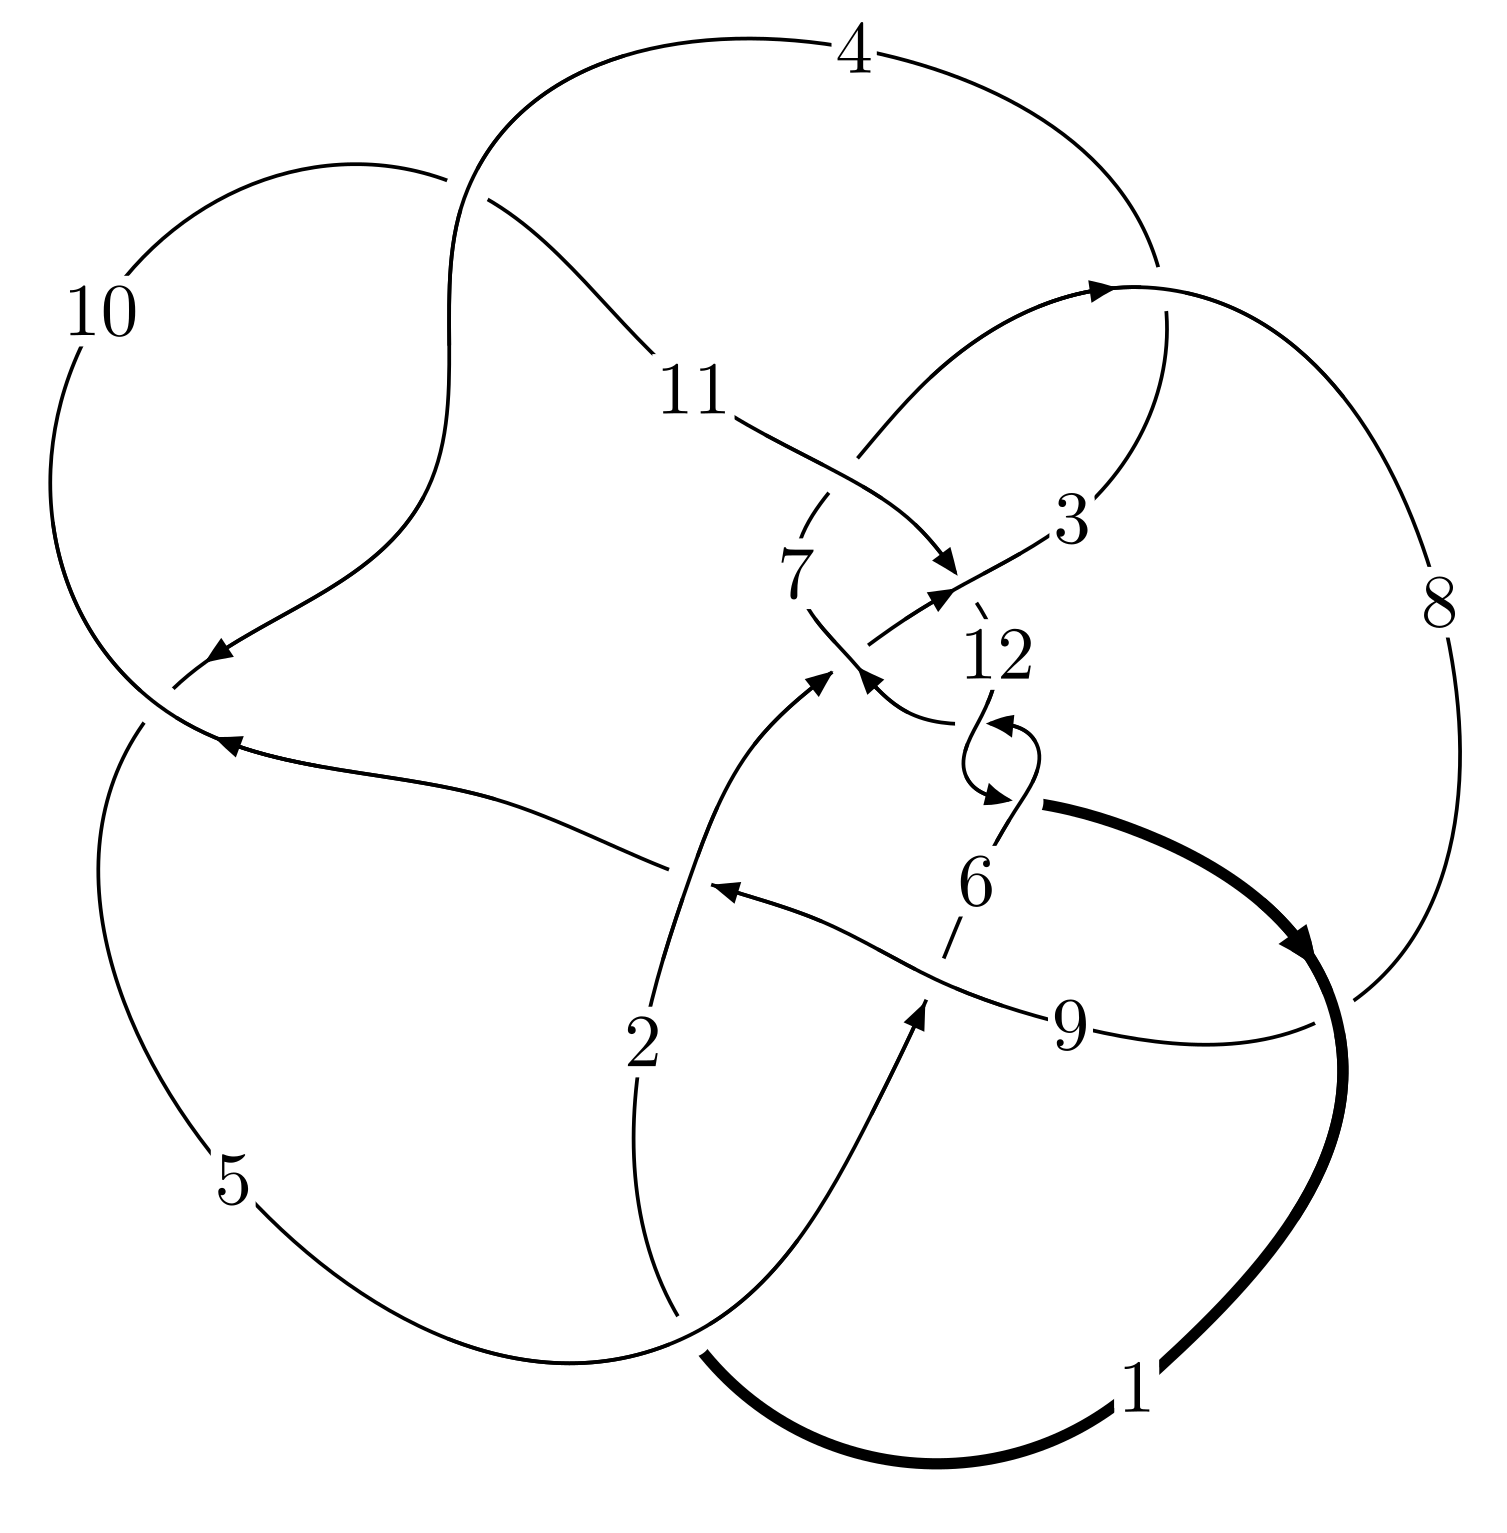
\includegraphics[width=112pt]{../../../GIT/diagram.site/Diagrams/png/2052_12a_1251.png}\\
\ \ \ A knot diagram\footnotemark}&
\allowdisplaybreaks
\textbf{Linearized knot diagam} \\
\cline{2-2}
 &
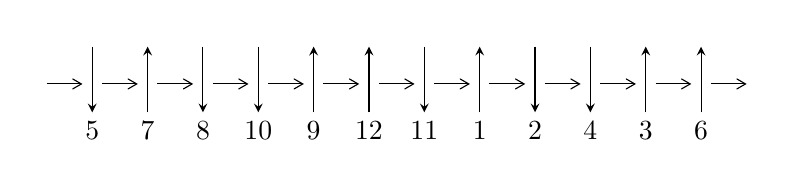
\begin{tikzpicture}[x=20pt, y=17pt]
	% nodes
	\node (C0) at (0, 0) {};
	\node (C1) at (1, 0) {};
	\node (C1U) at (1, +1) {};
	\node (C1D) at (1, -1) {5};

	\node (C2) at (2, 0) {};
	\node (C2U) at (2, +1) {};
	\node (C2D) at (2, -1) {7};

	\node (C3) at (3, 0) {};
	\node (C3U) at (3, +1) {};
	\node (C3D) at (3, -1) {8};

	\node (C4) at (4, 0) {};
	\node (C4U) at (4, +1) {};
	\node (C4D) at (4, -1) {10};

	\node (C5) at (5, 0) {};
	\node (C5U) at (5, +1) {};
	\node (C5D) at (5, -1) {9};

	\node (C6) at (6, 0) {};
	\node (C6U) at (6, +1) {};
	\node (C6D) at (6, -1) {12};

	\node (C7) at (7, 0) {};
	\node (C7U) at (7, +1) {};
	\node (C7D) at (7, -1) {11};

	\node (C8) at (8, 0) {};
	\node (C8U) at (8, +1) {};
	\node (C8D) at (8, -1) {1};

	\node (C9) at (9, 0) {};
	\node (C9U) at (9, +1) {};
	\node (C9D) at (9, -1) {2};

	\node (C10) at (10, 0) {};
	\node (C10U) at (10, +1) {};
	\node (C10D) at (10, -1) {4};

	\node (C11) at (11, 0) {};
	\node (C11U) at (11, +1) {};
	\node (C11D) at (11, -1) {3};

	\node (C12) at (12, 0) {};
	\node (C12U) at (12, +1) {};
	\node (C12D) at (12, -1) {6};
	\node (C13) at (13, 0) {};

	% arrows
	\draw[->,>={angle 60}]
	(C0) edge (C1) (C1) edge (C2) (C2) edge (C3) (C3) edge (C4) (C4) edge (C5) (C5) edge (C6) (C6) edge (C7) (C7) edge (C8) (C8) edge (C9) (C9) edge (C10) (C10) edge (C11) (C11) edge (C12) (C12) edge (C13) ;	\draw[->,>=stealth]
	(C1U) edge (C1D) (C2D) edge (C2U) (C3U) edge (C3D) (C4U) edge (C4D) (C5D) edge (C5U) (C6D) edge (C6U) (C7U) edge (C7D) (C8D) edge (C8U) (C9U) edge (C9D) (C10U) edge (C10D) (C11D) edge (C11U) (C12D) edge (C12U) ;
	\end{tikzpicture} \\
\hhline{~~} \\& 
\textbf{Solving Sequence} \\ \cline{2-2} 
 &
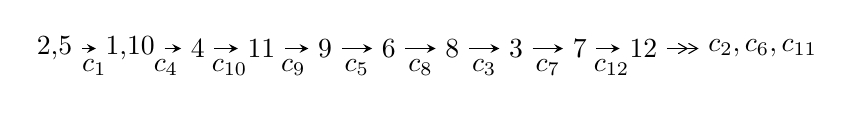
\begin{tikzpicture}[x=23pt, y=7pt]
	% node
	\node (A0) at (-1/8, 0) {2,5};
	\node (A1) at (17/16, 0) {1,10};
	\node (A2) at (17/8, 0) {4};
	\node (A3) at (25/8, 0) {11};
	\node (A4) at (33/8, 0) {9};
	\node (A5) at (41/8, 0) {6};
	\node (A6) at (49/8, 0) {8};
	\node (A7) at (57/8, 0) {3};
	\node (A8) at (65/8, 0) {7};
	\node (A9) at (73/8, 0) {12};
	\node (C1) at (1/2, -1) {$c_{1}$};
	\node (C2) at (13/8, -1) {$c_{4}$};
	\node (C3) at (21/8, -1) {$c_{10}$};
	\node (C4) at (29/8, -1) {$c_{9}$};
	\node (C5) at (37/8, -1) {$c_{5}$};
	\node (C6) at (45/8, -1) {$c_{8}$};
	\node (C7) at (53/8, -1) {$c_{3}$};
	\node (C8) at (61/8, -1) {$c_{7}$};
	\node (C9) at (69/8, -1) {$c_{12}$};
	\node (A10) at (11, 0) {$c_{2},c_{6},c_{11}$};

	% edge
	\draw[->,>=stealth]	
	(A0) edge (A1) (A1) edge (A2) (A2) edge (A3) (A3) edge (A4) (A4) edge (A5) (A5) edge (A6) (A6) edge (A7) (A7) edge (A8) (A8) edge (A9) ;
	\draw[->>,>={angle 60}]	
	(A9) edge (A10);
\end{tikzpicture} \\ 

\end{tabular} \\

\footnotetext{
The image of knot diagram is generated by the software ``\textbf{Draw programme}" developed by Andrew Bartholomew(\url{http://www.layer8.co.uk/maths/draw/index.htm\#Running-draw}), where we modified some parts for our purpose(\url{https://github.com/CATsTAILs/LinksPainter}).
}\phantom \\ \newline 
\centering \textbf{Ideals for irreducible components\footnotemark of $X_{\text{par}}$} 
 
\begin{align*}
I^u_{1}&=\langle 
5.41545\times10^{45} u^{37}+1.08996\times10^{47} u^{36}+\cdots+6.38981\times10^{46} b-4.06452\times10^{47},\\
\phantom{I^u_{1}}&\phantom{= \langle  }4.21436\times10^{47} u^{37}-5.72689\times10^{47} u^{36}+\cdots+6.38981\times10^{46} a-6.24484\times10^{47},\;u^{38}- u^{37}+\cdots-9 u-1\rangle \\
I^u_{2}&=\langle 
1.93258\times10^{942} u^{139}+1.35995\times10^{941} u^{138}+\cdots+1.25727\times10^{946} b+8.29635\times10^{946},\\
\phantom{I^u_{2}}&\phantom{= \langle  }-7.36045\times10^{947} u^{139}+2.14268\times10^{946} u^{138}+\cdots+1.30768\times10^{950} a+3.16361\times10^{951},\\
\phantom{I^u_{2}}&\phantom{= \langle  }u^{140}+12 u^{138}+\cdots+54306 u+10401\rangle \\
I^u_{3}&=\langle 
5.84926\times10^{78} u^{43}+2.23945\times10^{79} u^{42}+\cdots+7.36510\times10^{78} b+3.17801\times10^{79},\\
\phantom{I^u_{3}}&\phantom{= \langle  }-7.36354\times10^{78} u^{43}-2.10865\times10^{79} u^{42}+\cdots+2.45503\times10^{78} a-1.10180\times10^{79},\;u^{44}+3 u^{43}+\cdots+6 u+1\rangle \\
I^u_{4}&=\langle 
b+u,\;a,\;u^2- u+1\rangle \\
\\
\end{align*}
\raggedright * 4 irreducible components of $\dim_{\mathbb{C}}=0$, with total 224 representations.\\
\footnotetext{All coefficients of polynomials are rational numbers. But the coefficients are sometimes approximated in decimal forms when there is not enough margin.}
\newpage
\renewcommand{\arraystretch}{1}
\centering \section*{I. $I^u_{1}= \langle 5.42\times10^{45} u^{37}+1.09\times10^{47} u^{36}+\cdots+6.39\times10^{46} b-4.06\times10^{47},\;4.21\times10^{47} u^{37}-5.73\times10^{47} u^{36}+\cdots+6.39\times10^{46} a-6.24\times10^{47},\;u^{38}- u^{37}+\cdots-9 u-1 \rangle$}
\flushleft \textbf{(i) Arc colorings}\\
\begin{tabular}{m{7pt} m{180pt} m{7pt} m{180pt} }
\flushright $a_{2}=$&$\begin{pmatrix}1\\0\end{pmatrix}$ \\
\flushright $a_{5}=$&$\begin{pmatrix}0\\u\end{pmatrix}$ \\
\flushright $a_{1}=$&$\begin{pmatrix}1\\- u^2\end{pmatrix}$ \\
\flushright $a_{10}=$&$\begin{pmatrix}-6.59544 u^{37}+8.96254 u^{36}+\cdots+82.8273 u+9.77312\\-0.0847514 u^{37}-1.70577 u^{36}+\cdots+42.9121 u+6.36094\end{pmatrix}$ \\
\flushright $a_{4}=$&$\begin{pmatrix}-6.42624 u^{37}+9.22886 u^{36}+\cdots+19.2650 u+1.75561\\0.910048 u^{37}-2.06794 u^{36}+\cdots-2.54449 u-0.660358\end{pmatrix}$ \\
\flushright $a_{11}=$&$\begin{pmatrix}8.60481 u^{37}-10.8610 u^{36}+\cdots-101.127 u-12.6893\\-2.24228 u^{37}+1.54603 u^{36}+\cdots+55.9095 u+7.23400\end{pmatrix}$ \\
\flushright $a_{9}=$&$\begin{pmatrix}-6.68019 u^{37}+7.25676 u^{36}+\cdots+125.739 u+16.1341\\-0.0847514 u^{37}-1.70577 u^{36}+\cdots+42.9121 u+6.36094\end{pmatrix}$ \\
\flushright $a_{6}=$&$\begin{pmatrix}-7.56505 u^{37}+10.8064 u^{36}+\cdots-8.83701 u-3.28785\\-2.04886 u^{37}+3.64546 u^{36}+\cdots-23.5575 u-4.38310\end{pmatrix}$ \\
\flushright $a_{8}=$&$\begin{pmatrix}-7.23400 u^{37}+9.47628 u^{36}+\cdots+84.3183 u+9.19655\\-0.142437 u^{37}-0.423822 u^{36}+\cdots+28.4746 u+4.69524\end{pmatrix}$ \\
\flushright $a_{3}=$&$\begin{pmatrix}-4.16928 u^{37}+7.04773 u^{36}+\cdots-22.3735 u-2.69198\\3.39814 u^{37}-2.23185 u^{36}+\cdots-81.7143 u-11.1789\end{pmatrix}$ \\
\flushright $a_{7}=$&$\begin{pmatrix}-4.97785 u^{37}+9.43787 u^{36}+\cdots+19.5643 u+0.591739\\0.553812 u^{37}-2.21951 u^{36}+\cdots+41.4211 u+6.93751\end{pmatrix}$ \\
\flushright $a_{12}=$&$\begin{pmatrix}-0.515910 u^{37}+0.638113 u^{36}+\cdots-59.9990 u-12.7552\\-3.06293 u^{37}+4.04695 u^{36}+\cdots+17.0847 u+0.406432\end{pmatrix}$\\&\end{tabular}
\flushleft \textbf{(ii) Obstruction class $= -1$}\\~\\
\flushleft \textbf{(iii) Cusp Shapes $= -12.1292 u^{37}+7.88921 u^{36}+\cdots+89.0283 u+5.29741$}\\~\\
\newpage\renewcommand{\arraystretch}{1}
\flushleft \textbf{(iv) u-Polynomials at the component}\newline \\
\begin{tabular}{m{50pt}|m{274pt}}
Crossings & \hspace{64pt}u-Polynomials at each crossing \\
\hline $$\begin{aligned}c_{1},c_{7}\end{aligned}$$&$\begin{aligned}
&u^{38}+u^{37}+\cdots+9 u-1
\end{aligned}$\\
\hline $$\begin{aligned}c_{2},c_{8}\end{aligned}$$&$\begin{aligned}
&u^{38}+u^{37}+\cdots+3 u+1
\end{aligned}$\\
\hline $$\begin{aligned}c_{3},c_{9}\end{aligned}$$&$\begin{aligned}
&u^{38}- u^{37}+\cdots-3 u+1
\end{aligned}$\\
\hline $$\begin{aligned}c_{4},c_{10}\end{aligned}$$&$\begin{aligned}
&u^{38}-5 u^{37}+\cdots+1968 u-260
\end{aligned}$\\
\hline $$\begin{aligned}c_{5},c_{11}\end{aligned}$$&$\begin{aligned}
&u^{38}- u^{37}+\cdots-9 u-1
\end{aligned}$\\
\hline $$\begin{aligned}c_{6},c_{12}\end{aligned}$$&$\begin{aligned}
&u^{38}+5 u^{37}+\cdots-1968 u-260
\end{aligned}$\\
\hline
\end{tabular}\\~\\
\newpage\renewcommand{\arraystretch}{1}
\flushleft \textbf{(v) Riley Polynomials at the component}\newline \\
\begin{tabular}{m{50pt}|m{274pt}}
Crossings & \hspace{64pt}Riley Polynomials at each crossing \\
\hline $$\begin{aligned}c_{1},c_{5},c_{7}\\c_{11}\end{aligned}$$&$\begin{aligned}
&y^{38}-3 y^{37}+\cdots-7 y+1
\end{aligned}$\\
\hline $$\begin{aligned}c_{2},c_{3},c_{8}\\c_{9}\end{aligned}$$&$\begin{aligned}
&y^{38}+11 y^{37}+\cdots-9 y+1
\end{aligned}$\\
\hline $$\begin{aligned}c_{4},c_{6},c_{10}\\c_{12}\end{aligned}$$&$\begin{aligned}
&y^{38}+23 y^{37}+\cdots-657344 y+67600
\end{aligned}$\\
\hline
\end{tabular}\\~\\
\newpage\flushleft \textbf{(vi) Complex Volumes and Cusp Shapes}
$$\begin{array}{c|c|c}  
\text{Solutions to }I^u_{1}& \I (\text{vol} + \sqrt{-1}CS) & \text{Cusp shape}\\
 \hline 
\begin{aligned}
u &= \phantom{-}0.968211 + 0.099082 I \\
a &= \phantom{-}0.401521 - 0.037333 I \\
b &= -0.802971 - 0.684067 I\end{aligned}
 & -6.09133 + 2.82939 I & -12.39412 - 2.25794 I \\ \hline\begin{aligned}
u &= \phantom{-}0.968211 - 0.099082 I \\
a &= \phantom{-}0.401521 + 0.037333 I \\
b &= -0.802971 + 0.684067 I\end{aligned}
 & -6.09133 - 2.82939 I & -12.39412 + 2.25794 I \\ \hline\begin{aligned}
u &= \phantom{-}0.922908\phantom{ +0.000000I} \\
a &= -1.81558\phantom{ +0.000000I} \\
b &= \phantom{-}0.594003\phantom{ +0.000000I}\end{aligned}
 & -0.408756\phantom{ +0.000000I} & -21.5410\phantom{ +0.000000I} \\ \hline\begin{aligned}
u &= \phantom{-}0.720784 + 0.523136 I \\
a &= \phantom{-}0.55211 - 1.81656 I \\
b &= -0.618829 - 0.151609 I\end{aligned}
 & -4.50176 - 6.57911 I & -7.6096 + 11.9321 I \\ \hline\begin{aligned}
u &= \phantom{-}0.720784 - 0.523136 I \\
a &= \phantom{-}0.55211 + 1.81656 I \\
b &= -0.618829 + 0.151609 I\end{aligned}
 & -4.50176 + 6.57911 I & -7.6096 - 11.9321 I \\ \hline\begin{aligned}
u &= -1.12740\phantom{ +0.000000I} \\
a &= -1.26510\phantom{ +0.000000I} \\
b &= \phantom{-}0.446488\phantom{ +0.000000I}\end{aligned}
 & \phantom{-}0.408756\phantom{ +0.000000I} & \phantom{-}21.5410\phantom{ +0.000000I} \\ \hline\begin{aligned}
u &= -0.600621 + 0.958137 I \\
a &= \phantom{-}1.167140 - 0.465471 I \\
b &= -1.090910 + 0.751718 I\end{aligned}
 & \phantom{-}3.33253 + 3.84409 I & \phantom{-}1.41355 - 3.81235 I \\ \hline\begin{aligned}
u &= -0.600621 - 0.958137 I \\
a &= \phantom{-}1.167140 + 0.465471 I \\
b &= -1.090910 - 0.751718 I\end{aligned}
 & \phantom{-}3.33253 - 3.84409 I & \phantom{-}1.41355 + 3.81235 I \\ \hline\begin{aligned}
u &= \phantom{-}0.763304 + 0.285378 I \\
a &= -0.769399 + 0.299416 I \\
b &= \phantom{-}0.641337 + 0.167735 I\end{aligned}
 & -1.42108 - 0.29384 I & -6.42575 - 0.42207 I \\ \hline\begin{aligned}
u &= \phantom{-}0.763304 - 0.285378 I \\
a &= -0.769399 - 0.299416 I \\
b &= \phantom{-}0.641337 - 0.167735 I\end{aligned}
 & -1.42108 + 0.29384 I & -6.42575 + 0.42207 I\\
 \hline 
 \end{array}$$\newpage$$\begin{array}{c|c|c}  
\text{Solutions to }I^u_{1}& \I (\text{vol} + \sqrt{-1}CS) & \text{Cusp shape}\\
 \hline 
\begin{aligned}
u &= -0.313558 + 0.748788 I \\
a &= -1.84466 - 0.27944 I \\
b &= \phantom{-}0.107405 - 1.317060 I\end{aligned}
 & \phantom{-}3.85199 + 3.54385 I & \phantom{-}6.26632 - 12.05234 I \\ \hline\begin{aligned}
u &= -0.313558 - 0.748788 I \\
a &= -1.84466 + 0.27944 I \\
b &= \phantom{-}0.107405 + 1.317060 I\end{aligned}
 & \phantom{-}3.85199 - 3.54385 I & \phantom{-}6.26632 + 12.05234 I \\ \hline\begin{aligned}
u &= -0.317210 + 0.738243 I \\
a &= -1.62595 + 0.37185 I \\
b &= \phantom{-}1.03695 - 1.43027 I\end{aligned}
 & \phantom{-}6.09133 + 2.82939 I & \phantom{-}12.39412 - 2.25794 I \\ \hline\begin{aligned}
u &= -0.317210 - 0.738243 I \\
a &= -1.62595 - 0.37185 I \\
b &= \phantom{-}1.03695 + 1.43027 I\end{aligned}
 & \phantom{-}6.09133 - 2.82939 I & \phantom{-}12.39412 + 2.25794 I \\ \hline\begin{aligned}
u &= -0.969222 + 0.842096 I \\
a &= \phantom{-}0.963939 + 0.355295 I \\
b &= -0.824258 + 0.634902 I\end{aligned}
 & \phantom{-0.000000 -}8.69452 I & \phantom{-0.000000 } 0. - 12.41317 I \\ \hline\begin{aligned}
u &= -0.969222 - 0.842096 I \\
a &= \phantom{-}0.963939 - 0.355295 I \\
b &= -0.824258 - 0.634902 I\end{aligned}
 & \phantom{-0.000000 } -8.69452 I & \phantom{-0.000000 -}0. + 12.41317 I \\ \hline\begin{aligned}
u &= -0.276258 + 0.623777 I \\
a &= \phantom{-}1.67633 - 0.36759 I \\
b &= -0.67294 + 2.23248 I\end{aligned}
 & \phantom{-}2.19412 + 1.25898 I & \phantom{-}0.90146 - 4.40538 I \\ \hline\begin{aligned}
u &= -0.276258 - 0.623777 I \\
a &= \phantom{-}1.67633 + 0.36759 I \\
b &= -0.67294 - 2.23248 I\end{aligned}
 & \phantom{-}2.19412 - 1.25898 I & \phantom{-}0.90146 + 4.40538 I \\ \hline\begin{aligned}
u &= -0.922652 + 0.956457 I \\
a &= -0.870010 - 0.455985 I \\
b &= \phantom{-}1.098310 - 0.762936 I\end{aligned}
 & -6.0882 + 14.6929 I & -3.35386 - 10.24839 I \\ \hline\begin{aligned}
u &= -0.922652 - 0.956457 I \\
a &= -0.870010 + 0.455985 I \\
b &= \phantom{-}1.098310 + 0.762936 I\end{aligned}
 & -6.0882 - 14.6929 I & -3.35386 + 10.24839 I\\
 \hline 
 \end{array}$$\newpage$$\begin{array}{c|c|c}  
\text{Solutions to }I^u_{1}& \I (\text{vol} + \sqrt{-1}CS) & \text{Cusp shape}\\
 \hline 
\begin{aligned}
u &= -0.267862 + 0.556164 I \\
a &= \phantom{-}2.84678 - 0.60784 I \\
b &= -0.324135 + 0.855181 I\end{aligned}
 & \phantom{-}5.02615 + 1.33424 I & \phantom{-}10.68384 - 4.00875 I \\ \hline\begin{aligned}
u &= -0.267862 - 0.556164 I \\
a &= \phantom{-}2.84678 + 0.60784 I \\
b &= -0.324135 - 0.855181 I\end{aligned}
 & \phantom{-}5.02615 - 1.33424 I & \phantom{-}10.68384 + 4.00875 I \\ \hline\begin{aligned}
u &= -1.44047 + 0.11070 I \\
a &= -0.120309 + 0.887526 I \\
b &= \phantom{-}0.344050 - 1.303370 I\end{aligned}
 & -2.19412 - 1.25898 I & \phantom{-0.000000 } 0 \\ \hline\begin{aligned}
u &= -1.44047 - 0.11070 I \\
a &= -0.120309 - 0.887526 I \\
b &= \phantom{-}0.344050 + 1.303370 I\end{aligned}
 & -2.19412 + 1.25898 I & \phantom{-0.000000 } 0 \\ \hline\begin{aligned}
u &= -0.81328 + 1.33675 I \\
a &= -0.457106 + 0.006304 I \\
b &= \phantom{-}0.849741 - 0.044800 I\end{aligned}
 & -5.02615 - 1.33424 I & \phantom{-0.000000 } 0 \\ \hline\begin{aligned}
u &= -0.81328 - 1.33675 I \\
a &= -0.457106 - 0.006304 I \\
b &= \phantom{-}0.849741 + 0.044800 I\end{aligned}
 & -5.02615 + 1.33424 I & \phantom{-0.000000 } 0 \\ \hline\begin{aligned}
u &= \phantom{-}0.94529 + 1.26888 I \\
a &= \phantom{-}0.965645 + 0.331885 I \\
b &= -1.25182 - 1.29006 I\end{aligned}
 & \phantom{-0.000000 } -20.8093 I & \phantom{-0.000000 } 0 \\ \hline\begin{aligned}
u &= \phantom{-}0.94529 - 1.26888 I \\
a &= \phantom{-}0.965645 - 0.331885 I \\
b &= -1.25182 + 1.29006 I\end{aligned}
 & \phantom{-0.000000 -}20.8093 I & \phantom{-0.000000 } 0 \\ \hline\begin{aligned}
u &= -0.231065 + 0.320032 I \\
a &= -0.17217 - 1.64494 I \\
b &= -0.373634 - 0.346076 I\end{aligned}
 & \phantom{-}1.42108 + 0.29384 I & \phantom{-}6.42575 + 0.42207 I \\ \hline\begin{aligned}
u &= -0.231065 - 0.320032 I \\
a &= -0.17217 + 1.64494 I \\
b &= -0.373634 + 0.346076 I\end{aligned}
 & \phantom{-}1.42108 - 0.29384 I & \phantom{-}6.42575 - 0.42207 I\\
 \hline 
 \end{array}$$\newpage$$\begin{array}{c|c|c}  
\text{Solutions to }I^u_{1}& \I (\text{vol} + \sqrt{-1}CS) & \text{Cusp shape}\\
 \hline 
\begin{aligned}
u &= \phantom{-}0.95520 + 1.34300 I \\
a &= -0.919074 - 0.295860 I \\
b &= \phantom{-}1.06753 + 1.08845 I\end{aligned}
 & \phantom{-}6.0882 - 14.6929 I & \phantom{-0.000000 } 0 \\ \hline\begin{aligned}
u &= \phantom{-}0.95520 - 1.34300 I \\
a &= -0.919074 + 0.295860 I \\
b &= \phantom{-}1.06753 - 1.08845 I\end{aligned}
 & \phantom{-}6.0882 + 14.6929 I & \phantom{-0.000000 } 0 \\ \hline\begin{aligned}
u &= -0.320051 + 0.098884 I \\
a &= \phantom{-}0.06483 + 2.75766 I \\
b &= \phantom{-}0.803936 + 0.504458 I\end{aligned}
 & -3.33253 + 3.84409 I & -1.41355 - 3.81235 I \\ \hline\begin{aligned}
u &= -0.320051 - 0.098884 I \\
a &= \phantom{-}0.06483 - 2.75766 I \\
b &= \phantom{-}0.803936 - 0.504458 I\end{aligned}
 & -3.33253 - 3.84409 I & -1.41355 + 3.81235 I \\ \hline\begin{aligned}
u &= \phantom{-}0.98153 + 1.45353 I \\
a &= \phantom{-}0.831832 + 0.178309 I \\
b &= -0.849035 - 0.685813 I\end{aligned}
 & \phantom{-}4.50176 - 6.57911 I & \phantom{-0.000000 } 0 \\ \hline\begin{aligned}
u &= \phantom{-}0.98153 - 1.45353 I \\
a &= \phantom{-}0.831832 - 0.178309 I \\
b &= -0.849035 + 0.685813 I\end{aligned}
 & \phantom{-}4.50176 + 6.57911 I & \phantom{-0.000000 } 0 \\ \hline\begin{aligned}
u &= \phantom{-}1.74017 + 0.80024 I \\
a &= -0.151098 - 0.523665 I \\
b &= -0.160972 + 0.236880 I\end{aligned}
 & -3.85199 + 3.54385 I & \phantom{-0.000000 } 0 \\ \hline\begin{aligned}
u &= \phantom{-}1.74017 - 0.80024 I \\
a &= -0.151098 + 0.523665 I \\
b &= -0.160972 - 0.236880 I\end{aligned}
 & -3.85199 - 3.54385 I & \phantom{-0.000000 } 0\\
 \hline 
 \end{array}$$\newpage\newpage\renewcommand{\arraystretch}{1}
\centering \section*{II. $I^u_{2}= \langle 1.93\times10^{942} u^{139}+1.36\times10^{941} u^{138}+\cdots+1.26\times10^{946} b+8.30\times10^{946},\;-7.36\times10^{947} u^{139}+2.14\times10^{946} u^{138}+\cdots+1.31\times10^{950} a+3.16\times10^{951},\;u^{140}+12 u^{138}+\cdots+54306 u+10401 \rangle$}
\flushleft \textbf{(i) Arc colorings}\\
\begin{tabular}{m{7pt} m{180pt} m{7pt} m{180pt} }
\flushright $a_{2}=$&$\begin{pmatrix}1\\0\end{pmatrix}$ \\
\flushright $a_{5}=$&$\begin{pmatrix}0\\u\end{pmatrix}$ \\
\flushright $a_{1}=$&$\begin{pmatrix}1\\- u^2\end{pmatrix}$ \\
\flushright $a_{10}=$&$\begin{pmatrix}0.00562862 u^{139}-0.000163853 u^{138}+\cdots+116.482 u-24.1925\\-0.000153713 u^{139}-0.0000108168 u^{138}+\cdots-51.8041 u-6.59872\end{pmatrix}$ \\
\flushright $a_{4}=$&$\begin{pmatrix}0.00582107 u^{139}-0.00216164 u^{138}+\cdots-297.717 u-83.6275\\-0.00138482 u^{139}-0.000452467 u^{138}+\cdots-181.344 u-19.2547\end{pmatrix}$ \\
\flushright $a_{11}=$&$\begin{pmatrix}0.00272863 u^{139}-0.00304649 u^{138}+\cdots-576.031 u-104.088\\0.000334281 u^{139}-0.000906312 u^{138}+\cdots-62.9029 u-15.7146\end{pmatrix}$ \\
\flushright $a_{9}=$&$\begin{pmatrix}0.00547491 u^{139}-0.000174670 u^{138}+\cdots+64.6777 u-30.7912\\-0.000153713 u^{139}-0.0000108168 u^{138}+\cdots-51.8041 u-6.59872\end{pmatrix}$ \\
\flushright $a_{6}=$&$\begin{pmatrix}0.00446024 u^{139}-0.00295521 u^{138}+\cdots-561.134 u-115.140\\0.0000239840 u^{139}-0.000341102 u^{138}+\cdots-80.0729 u-12.2574\end{pmatrix}$ \\
\flushright $a_{8}=$&$\begin{pmatrix}0.00727880 u^{139}+0.0000415565 u^{138}+\cdots+163.941 u-26.0092\\0.000511692 u^{139}+0.0000718818 u^{138}+\cdots-21.2994 u-4.34975\end{pmatrix}$ \\
\flushright $a_{3}=$&$\begin{pmatrix}0.00444084 u^{139}-0.00312167 u^{138}+\cdots-550.988 u-107.315\\0.000929956 u^{139}-0.0000740184 u^{138}+\cdots-10.8583 u-4.88679\end{pmatrix}$ \\
\flushright $a_{7}=$&$\begin{pmatrix}-0.00462116 u^{139}+0.0000891687 u^{138}+\cdots+177.520 u+47.1196\\-0.000737727 u^{139}-0.000616594 u^{138}+\cdots-91.7030 u-13.5757\end{pmatrix}$ \\
\flushright $a_{12}=$&$\begin{pmatrix}-0.000463728 u^{139}-0.00480298 u^{138}+\cdots-881.879 u-163.598\\-0.00146877 u^{139}-0.00111609 u^{138}+\cdots-227.563 u-36.3600\end{pmatrix}$\\&\end{tabular}
\flushleft \textbf{(ii) Obstruction class $= -1$}\\~\\
\flushleft \textbf{(iii) Cusp Shapes $= -0.00535623 u^{139}-0.00670142 u^{138}+\cdots-1311.85 u-217.480$}\\~\\
\newpage\renewcommand{\arraystretch}{1}
\flushleft \textbf{(iv) u-Polynomials at the component}\newline \\
\begin{tabular}{m{50pt}|m{274pt}}
Crossings & \hspace{64pt}u-Polynomials at each crossing \\
\hline $$\begin{aligned}c_{1},c_{7}\end{aligned}$$&$\begin{aligned}
&u^{140}+12 u^{138}+\cdots-54306 u+10401
\end{aligned}$\\
\hline $$\begin{aligned}c_{2},c_{8}\end{aligned}$$&$\begin{aligned}
&u^{140}+u^{139}+\cdots-96505 u+4729
\end{aligned}$\\
\hline $$\begin{aligned}c_{3},c_{9}\end{aligned}$$&$\begin{aligned}
&u^{140}- u^{139}+\cdots+96505 u+4729
\end{aligned}$\\
\hline $$\begin{aligned}c_{4},c_{10}\end{aligned}$$&$\begin{aligned}
&(u^{70}+2 u^{69}+\cdots+1179 u-211)^{2}
\end{aligned}$\\
\hline $$\begin{aligned}c_{5},c_{11}\end{aligned}$$&$\begin{aligned}
&u^{140}+12 u^{138}+\cdots+54306 u+10401
\end{aligned}$\\
\hline $$\begin{aligned}c_{6},c_{12}\end{aligned}$$&$\begin{aligned}
&(u^{70}-2 u^{69}+\cdots-1179 u-211)^{2}
\end{aligned}$\\
\hline
\end{tabular}\\~\\
\newpage\renewcommand{\arraystretch}{1}
\flushleft \textbf{(v) Riley Polynomials at the component}\newline \\
\begin{tabular}{m{50pt}|m{274pt}}
Crossings & \hspace{64pt}Riley Polynomials at each crossing \\
\hline $$\begin{aligned}c_{1},c_{5},c_{7}\\c_{11}\end{aligned}$$&$\begin{aligned}
&y^{140}+24 y^{139}+\cdots+6449867628 y+108180801
\end{aligned}$\\
\hline $$\begin{aligned}c_{2},c_{3},c_{8}\\c_{9}\end{aligned}$$&$\begin{aligned}
&y^{140}+33 y^{139}+\cdots-890326919 y+22363441
\end{aligned}$\\
\hline $$\begin{aligned}c_{4},c_{6},c_{10}\\c_{12}\end{aligned}$$&$\begin{aligned}
&(y^{70}+50 y^{69}+\cdots-865495 y+44521)^{2}
\end{aligned}$\\
\hline
\end{tabular}\\~\\
\newpage\flushleft \textbf{(vi) Complex Volumes and Cusp Shapes}
$$\begin{array}{c|c|c}  
\text{Solutions to }I^u_{2}& \I (\text{vol} + \sqrt{-1}CS) & \text{Cusp shape}\\
 \hline 
\begin{aligned}
u &= -0.260607 + 0.957647 I \\
a &= \phantom{-}1.076760 - 0.047164 I \\
b &= -0.17973 + 1.61195 I\end{aligned}
 & \phantom{-}3.61200 + 0.98906 I & \phantom{-0.000000 } 0 \\ \hline\begin{aligned}
u &= -0.260607 - 0.957647 I \\
a &= \phantom{-}1.076760 + 0.047164 I \\
b &= -0.17973 - 1.61195 I\end{aligned}
 & \phantom{-}3.61200 - 0.98906 I & \phantom{-0.000000 } 0 \\ \hline\begin{aligned}
u &= \phantom{-}0.315607 + 0.938612 I \\
a &= -1.310900 + 0.087179 I \\
b &= \phantom{-}0.404767 + 0.995005 I\end{aligned}
 & \phantom{-0.000000 } -4.95068 I & \phantom{-0.000000 } 0 \\ \hline\begin{aligned}
u &= \phantom{-}0.315607 - 0.938612 I \\
a &= -1.310900 - 0.087179 I \\
b &= \phantom{-}0.404767 - 0.995005 I\end{aligned}
 & \phantom{-0.000000 -}4.95068 I & \phantom{-0.000000 } 0 \\ \hline\begin{aligned}
u &= \phantom{-}0.390897 + 0.900603 I \\
a &= \phantom{-}1.61401 + 0.05652 I \\
b &= -0.384643 - 1.255120 I\end{aligned}
 & \phantom{-}2.07145 - 12.42820 I & \phantom{-0.000000 } 0 \\ \hline\begin{aligned}
u &= \phantom{-}0.390897 - 0.900603 I \\
a &= \phantom{-}1.61401 - 0.05652 I \\
b &= -0.384643 + 1.255120 I\end{aligned}
 & \phantom{-}2.07145 + 12.42820 I & \phantom{-0.000000 } 0 \\ \hline\begin{aligned}
u &= \phantom{-}0.845309 + 0.568360 I \\
a &= \phantom{-}0.942280 + 0.931931 I \\
b &= -0.89869 - 1.69407 I\end{aligned}
 & \phantom{-}2.81456 - 7.38758 I & \phantom{-0.000000 } 0 \\ \hline\begin{aligned}
u &= \phantom{-}0.845309 - 0.568360 I \\
a &= \phantom{-}0.942280 - 0.931931 I \\
b &= -0.89869 + 1.69407 I\end{aligned}
 & \phantom{-}2.81456 + 7.38758 I & \phantom{-0.000000 } 0 \\ \hline\begin{aligned}
u &= -0.967287 + 0.122879 I \\
a &= \phantom{-}0.003203 + 1.226480 I \\
b &= \phantom{-}0.329864 - 0.011835 I\end{aligned}
 & -3.10613 + 3.74546 I & \phantom{-0.000000 } 0 \\ \hline\begin{aligned}
u &= -0.967287 - 0.122879 I \\
a &= \phantom{-}0.003203 - 1.226480 I \\
b &= \phantom{-}0.329864 + 0.011835 I\end{aligned}
 & -3.10613 - 3.74546 I & \phantom{-0.000000 } 0\\
 \hline 
 \end{array}$$\newpage$$\begin{array}{c|c|c}  
\text{Solutions to }I^u_{2}& \I (\text{vol} + \sqrt{-1}CS) & \text{Cusp shape}\\
 \hline 
\begin{aligned}
u &= -0.685126 + 0.772834 I \\
a &= -1.23616 + 0.88689 I \\
b &= \phantom{-}0.030831 - 0.820977 I\end{aligned}
 & \phantom{-}3.53444 + 0.13727 I & \phantom{-0.000000 } 0 \\ \hline\begin{aligned}
u &= -0.685126 - 0.772834 I \\
a &= -1.23616 - 0.88689 I \\
b &= \phantom{-}0.030831 + 0.820977 I\end{aligned}
 & \phantom{-}3.53444 - 0.13727 I & \phantom{-0.000000 } 0 \\ \hline\begin{aligned}
u &= -0.559810 + 0.759792 I \\
a &= -0.029368 - 0.290599 I \\
b &= \phantom{-}0.196776 - 0.949676 I\end{aligned}
 & \phantom{-}1.99898 + 2.39251 I & \phantom{-0.000000 } 0 \\ \hline\begin{aligned}
u &= -0.559810 - 0.759792 I \\
a &= -0.029368 + 0.290599 I \\
b &= \phantom{-}0.196776 + 0.949676 I\end{aligned}
 & \phantom{-}1.99898 - 2.39251 I & \phantom{-0.000000 } 0 \\ \hline\begin{aligned}
u &= \phantom{-}0.580972 + 0.722903 I \\
a &= \phantom{-}0.335188 - 0.330442 I \\
b &= -0.337362 + 0.975889 I\end{aligned}
 & \phantom{-}1.42365 - 4.02526 I & \phantom{-0.000000 } 0 \\ \hline\begin{aligned}
u &= \phantom{-}0.580972 - 0.722903 I \\
a &= \phantom{-}0.335188 + 0.330442 I \\
b &= -0.337362 - 0.975889 I\end{aligned}
 & \phantom{-}1.42365 + 4.02526 I & \phantom{-0.000000 } 0 \\ \hline\begin{aligned}
u &= \phantom{-}0.449147 + 0.980408 I \\
a &= \phantom{-}0.209901 - 0.346117 I \\
b &= -0.708833 - 0.783820 I\end{aligned}
 & \phantom{-}1.42365 - 4.02526 I & \phantom{-0.000000 } 0 \\ \hline\begin{aligned}
u &= \phantom{-}0.449147 - 0.980408 I \\
a &= \phantom{-}0.209901 + 0.346117 I \\
b &= -0.708833 + 0.783820 I\end{aligned}
 & \phantom{-}1.42365 + 4.02526 I & \phantom{-0.000000 } 0 \\ \hline\begin{aligned}
u &= -0.392217 + 1.008780 I \\
a &= -0.200302 - 0.157294 I \\
b &= \phantom{-}0.133244 + 0.765577 I\end{aligned}
 & \phantom{-}1.99898 - 2.39251 I & \phantom{-0.000000 } 0 \\ \hline\begin{aligned}
u &= -0.392217 - 1.008780 I \\
a &= -0.200302 + 0.157294 I \\
b &= \phantom{-}0.133244 - 0.765577 I\end{aligned}
 & \phantom{-}1.99898 + 2.39251 I & \phantom{-0.000000 } 0\\
 \hline 
 \end{array}$$\newpage$$\begin{array}{c|c|c}  
\text{Solutions to }I^u_{2}& \I (\text{vol} + \sqrt{-1}CS) & \text{Cusp shape}\\
 \hline 
\begin{aligned}
u &= -0.351304 + 0.842177 I \\
a &= \phantom{-}1.51267 - 0.82276 I \\
b &= -0.150332 + 0.267043 I\end{aligned}
 & \phantom{-}3.53444 - 0.13727 I & \phantom{-0.000000 } 0 \\ \hline\begin{aligned}
u &= -0.351304 - 0.842177 I \\
a &= \phantom{-}1.51267 + 0.82276 I \\
b &= -0.150332 - 0.267043 I\end{aligned}
 & \phantom{-}3.53444 + 0.13727 I & \phantom{-0.000000 } 0 \\ \hline\begin{aligned}
u &= -0.542115 + 0.715651 I \\
a &= \phantom{-}0.049500 - 1.400900 I \\
b &= \phantom{-}0.859124 - 0.459279 I\end{aligned}
 & -5.16564 - 3.33643 I & \phantom{-0.000000 } 0 \\ \hline\begin{aligned}
u &= -0.542115 - 0.715651 I \\
a &= \phantom{-}0.049500 + 1.400900 I \\
b &= \phantom{-}0.859124 + 0.459279 I\end{aligned}
 & -5.16564 + 3.33643 I & \phantom{-0.000000 } 0 \\ \hline\begin{aligned}
u &= \phantom{-}0.252790 + 1.081740 I \\
a &= \phantom{-}1.123190 + 0.239963 I \\
b &= -0.207075 - 0.756252 I\end{aligned}
 & \phantom{-}5.37530 + 2.73843 I & \phantom{-0.000000 } 0 \\ \hline\begin{aligned}
u &= \phantom{-}0.252790 - 1.081740 I \\
a &= \phantom{-}1.123190 - 0.239963 I \\
b &= -0.207075 + 0.756252 I\end{aligned}
 & \phantom{-}5.37530 - 2.73843 I & \phantom{-0.000000 } 0 \\ \hline\begin{aligned}
u &= -0.425482 + 0.780133 I \\
a &= \phantom{-}1.52214 - 0.52417 I \\
b &= -1.78000 + 0.70554 I\end{aligned}
 & \phantom{-}3.10613 + 3.74546 I & \phantom{-0.000000 } 0 \\ \hline\begin{aligned}
u &= -0.425482 - 0.780133 I \\
a &= \phantom{-}1.52214 + 0.52417 I \\
b &= -1.78000 - 0.70554 I\end{aligned}
 & \phantom{-}3.10613 - 3.74546 I & \phantom{-0.000000 } 0 \\ \hline\begin{aligned}
u &= \phantom{-}0.732165 + 0.841538 I \\
a &= -0.747634 + 0.323942 I \\
b &= \phantom{-}1.196470 + 0.086638 I\end{aligned}
 & -2.58879 - 0.27761 I & \phantom{-0.000000 } 0 \\ \hline\begin{aligned}
u &= \phantom{-}0.732165 - 0.841538 I \\
a &= -0.747634 - 0.323942 I \\
b &= \phantom{-}1.196470 - 0.086638 I\end{aligned}
 & -2.58879 + 0.27761 I & \phantom{-0.000000 } 0\\
 \hline 
 \end{array}$$\newpage$$\begin{array}{c|c|c}  
\text{Solutions to }I^u_{2}& \I (\text{vol} + \sqrt{-1}CS) & \text{Cusp shape}\\
 \hline 
\begin{aligned}
u &= -0.257395 + 0.819091 I \\
a &= \phantom{-}1.36106 - 0.62195 I \\
b &= -1.14289 + 1.39217 I\end{aligned}
 & \phantom{-}6.17925 + 0.85610 I & \phantom{-0.000000 } 0 \\ \hline\begin{aligned}
u &= -0.257395 - 0.819091 I \\
a &= \phantom{-}1.36106 + 0.62195 I \\
b &= -1.14289 - 1.39217 I\end{aligned}
 & \phantom{-}6.17925 - 0.85610 I & \phantom{-0.000000 } 0 \\ \hline\begin{aligned}
u &= -0.535561 + 0.661055 I \\
a &= \phantom{-}0.083913 + 1.082100 I \\
b &= -0.653843 + 0.804828 I\end{aligned}
 & -5.37530 + 2.73843 I & \phantom{-0.000000 } 0 \\ \hline\begin{aligned}
u &= -0.535561 - 0.661055 I \\
a &= \phantom{-}0.083913 - 1.082100 I \\
b &= -0.653843 - 0.804828 I\end{aligned}
 & -5.37530 - 2.73843 I & \phantom{-0.000000 } 0 \\ \hline\begin{aligned}
u &= \phantom{-}0.801077 + 0.270434 I \\
a &= -0.83332 - 1.45240 I \\
b &= \phantom{-}1.20701 + 1.95684 I\end{aligned}
 & -0.55813 - 9.85968 I & \phantom{-0.000000 } 0 \\ \hline\begin{aligned}
u &= \phantom{-}0.801077 - 0.270434 I \\
a &= -0.83332 + 1.45240 I \\
b &= \phantom{-}1.20701 - 1.95684 I\end{aligned}
 & -0.55813 + 9.85968 I & \phantom{-0.000000 } 0 \\ \hline\begin{aligned}
u &= \phantom{-}0.790072 + 0.860480 I \\
a &= -0.109716 + 0.782801 I \\
b &= \phantom{-}0.938165 - 0.315917 I\end{aligned}
 & -5.37530 - 2.73843 I & \phantom{-0.000000 } 0 \\ \hline\begin{aligned}
u &= \phantom{-}0.790072 - 0.860480 I \\
a &= -0.109716 - 0.782801 I \\
b &= \phantom{-}0.938165 + 0.315917 I\end{aligned}
 & -5.37530 + 2.73843 I & \phantom{-0.000000 } 0 \\ \hline\begin{aligned}
u &= \phantom{-}0.524348 + 1.048140 I \\
a &= \phantom{-}0.029965 + 0.428280 I \\
b &= \phantom{-}0.852322 + 0.746485 I\end{aligned}
 & -2.81456 - 7.38758 I & \phantom{-0.000000 } 0 \\ \hline\begin{aligned}
u &= \phantom{-}0.524348 - 1.048140 I \\
a &= \phantom{-}0.029965 - 0.428280 I \\
b &= \phantom{-}0.852322 - 0.746485 I\end{aligned}
 & -2.81456 + 7.38758 I & \phantom{-0.000000 } 0\\
 \hline 
 \end{array}$$\newpage$$\begin{array}{c|c|c}  
\text{Solutions to }I^u_{2}& \I (\text{vol} + \sqrt{-1}CS) & \text{Cusp shape}\\
 \hline 
\begin{aligned}
u &= \phantom{-}0.274817 + 0.772107 I \\
a &= -0.786101 + 0.782232 I \\
b &= \phantom{-}0.184822 + 0.577082 I\end{aligned}
 & -2.58879 - 0.27761 I & \phantom{-0.000000 } 0 \\ \hline\begin{aligned}
u &= \phantom{-}0.274817 - 0.772107 I \\
a &= -0.786101 - 0.782232 I \\
b &= \phantom{-}0.184822 - 0.577082 I\end{aligned}
 & -2.58879 + 0.27761 I & \phantom{-0.000000 } 0 \\ \hline\begin{aligned}
u &= \phantom{-}0.848636 + 0.821513 I \\
a &= -0.795598 + 0.027066 I \\
b &= \phantom{-}0.902479 + 0.764781 I\end{aligned}
 & -1.99898 - 2.39251 I & \phantom{-0.000000 } 0 \\ \hline\begin{aligned}
u &= \phantom{-}0.848636 - 0.821513 I \\
a &= -0.795598 - 0.027066 I \\
b &= \phantom{-}0.902479 - 0.764781 I\end{aligned}
 & -1.99898 + 2.39251 I & \phantom{-0.000000 } 0 \\ \hline\begin{aligned}
u &= -0.002098 + 1.185280 I \\
a &= -1.267330 - 0.044236 I \\
b &= \phantom{-}0.144454 + 0.160431 I\end{aligned}
 & \phantom{-}3.75251 + 6.23561 I & \phantom{-0.000000 } 0 \\ \hline\begin{aligned}
u &= -0.002098 - 1.185280 I \\
a &= -1.267330 + 0.044236 I \\
b &= \phantom{-}0.144454 - 0.160431 I\end{aligned}
 & \phantom{-}3.75251 - 6.23561 I & \phantom{-0.000000 } 0 \\ \hline\begin{aligned}
u &= \phantom{-}0.245867 + 0.769791 I \\
a &= -2.03841 - 0.02255 I \\
b &= \phantom{-}0.453064 + 0.862653 I\end{aligned}
 & \phantom{-}6.07769 - 7.63458 I & \phantom{-0.000000 } 0 \\ \hline\begin{aligned}
u &= \phantom{-}0.245867 - 0.769791 I \\
a &= -2.03841 + 0.02255 I \\
b &= \phantom{-}0.453064 - 0.862653 I\end{aligned}
 & \phantom{-}6.07769 + 7.63458 I & \phantom{-0.000000 } 0 \\ \hline\begin{aligned}
u &= \phantom{-}1.186010 + 0.149076 I \\
a &= -0.046126 - 0.980985 I \\
b &= -0.14851 + 1.58671 I\end{aligned}
 & -3.61200 + 0.98906 I & \phantom{-0.000000 } 0 \\ \hline\begin{aligned}
u &= \phantom{-}1.186010 - 0.149076 I \\
a &= -0.046126 + 0.980985 I \\
b &= -0.14851 - 1.58671 I\end{aligned}
 & -3.61200 - 0.98906 I & \phantom{-0.000000 } 0\\
 \hline 
 \end{array}$$\newpage$$\begin{array}{c|c|c}  
\text{Solutions to }I^u_{2}& \I (\text{vol} + \sqrt{-1}CS) & \text{Cusp shape}\\
 \hline 
\begin{aligned}
u &= -0.856067 + 0.834835 I \\
a &= \phantom{-}0.553916 + 0.576593 I \\
b &= -0.758993 + 0.732139 I\end{aligned}
 & -6.07769 + 7.63458 I & \phantom{-0.000000 } 0 \\ \hline\begin{aligned}
u &= -0.856067 - 0.834835 I \\
a &= \phantom{-}0.553916 - 0.576593 I \\
b &= -0.758993 - 0.732139 I\end{aligned}
 & -6.07769 - 7.63458 I & \phantom{-0.000000 } 0 \\ \hline\begin{aligned}
u &= \phantom{-}0.822452 + 0.885058 I \\
a &= \phantom{-}0.725507 - 0.856629 I \\
b &= -1.092770 - 0.474982 I\end{aligned}
 & -2.64550 - 5.63372 I & \phantom{-0.000000 } 0 \\ \hline\begin{aligned}
u &= \phantom{-}0.822452 - 0.885058 I \\
a &= \phantom{-}0.725507 + 0.856629 I \\
b &= -1.092770 + 0.474982 I\end{aligned}
 & -2.64550 + 5.63372 I & \phantom{-0.000000 } 0 \\ \hline\begin{aligned}
u &= \phantom{-}0.829334 + 0.888333 I \\
a &= -0.796515 - 0.482925 I \\
b &= \phantom{-}0.85173 + 1.62859 I\end{aligned}
 & -3.75251 - 6.23561 I & \phantom{-0.000000 } 0 \\ \hline\begin{aligned}
u &= \phantom{-}0.829334 - 0.888333 I \\
a &= -0.796515 + 0.482925 I \\
b &= \phantom{-}0.85173 - 1.62859 I\end{aligned}
 & -3.75251 + 6.23561 I & \phantom{-0.000000 } 0 \\ \hline\begin{aligned}
u &= -1.214780 + 0.090690 I \\
a &= -0.351160 + 1.001060 I \\
b &= \phantom{-}0.078998 - 0.385780 I\end{aligned}
 & \phantom{-}2.58879 - 0.27761 I & \phantom{-0.000000 } 0 \\ \hline\begin{aligned}
u &= -1.214780 - 0.090690 I \\
a &= -0.351160 - 1.001060 I \\
b &= \phantom{-}0.078998 + 0.385780 I\end{aligned}
 & \phantom{-}2.58879 + 0.27761 I & \phantom{-0.000000 } 0 \\ \hline\begin{aligned}
u &= \phantom{-}0.470023 + 0.619470 I \\
a &= -0.074483 + 0.642767 I \\
b &= \phantom{-}0.14929 - 1.95058 I\end{aligned}
 & -2.81456 - 7.38758 I & \phantom{-0.000000 } 0 \\ \hline\begin{aligned}
u &= \phantom{-}0.470023 - 0.619470 I \\
a &= -0.074483 - 0.642767 I \\
b &= \phantom{-}0.14929 + 1.95058 I\end{aligned}
 & -2.81456 + 7.38758 I & \phantom{-0.000000 } 0\\
 \hline 
 \end{array}$$\newpage$$\begin{array}{c|c|c}  
\text{Solutions to }I^u_{2}& \I (\text{vol} + \sqrt{-1}CS) & \text{Cusp shape}\\
 \hline 
\begin{aligned}
u &= -0.152637 + 0.759225 I \\
a &= -1.65449 + 0.12307 I \\
b &= \phantom{-}0.286800 - 1.290370 I\end{aligned}
 & \phantom{-}6.17925 - 0.85610 I & \phantom{-0.000000 } 0 \\ \hline\begin{aligned}
u &= -0.152637 - 0.759225 I \\
a &= -1.65449 - 0.12307 I \\
b &= \phantom{-}0.286800 + 1.290370 I\end{aligned}
 & \phantom{-}6.17925 + 0.85610 I & \phantom{-0.000000 } 0 \\ \hline\begin{aligned}
u &= -0.471425 + 1.133980 I \\
a &= \phantom{-}1.135180 - 0.261406 I \\
b &= -0.925210 + 1.027120 I\end{aligned}
 & \phantom{-}3.10613 + 3.74546 I & \phantom{-0.000000 } 0 \\ \hline\begin{aligned}
u &= -0.471425 - 1.133980 I \\
a &= \phantom{-}1.135180 + 0.261406 I \\
b &= -0.925210 - 1.027120 I\end{aligned}
 & \phantom{-}3.10613 - 3.74546 I & \phantom{-0.000000 } 0 \\ \hline\begin{aligned}
u &= -0.321138 + 0.689372 I \\
a &= -1.112990 + 0.860013 I \\
b &= \phantom{-}0.63215 - 2.35643 I\end{aligned}
 & \phantom{-}3.61200 - 0.98906 I & \phantom{-0.000000 } 0 \\ \hline\begin{aligned}
u &= -0.321138 - 0.689372 I \\
a &= -1.112990 - 0.860013 I \\
b &= \phantom{-}0.63215 + 2.35643 I\end{aligned}
 & \phantom{-}3.61200 + 0.98906 I & \phantom{-0.000000 } 0 \\ \hline\begin{aligned}
u &= \phantom{-}0.817302 + 0.936461 I \\
a &= \phantom{-}0.997986 - 0.170928 I \\
b &= -1.23638 - 1.10075 I\end{aligned}
 & -5.16564 - 3.33643 I & \phantom{-0.000000 } 0 \\ \hline\begin{aligned}
u &= \phantom{-}0.817302 - 0.936461 I \\
a &= \phantom{-}0.997986 + 0.170928 I \\
b &= -1.23638 + 1.10075 I\end{aligned}
 & -5.16564 + 3.33643 I & \phantom{-0.000000 } 0 \\ \hline\begin{aligned}
u &= \phantom{-}0.774862 + 0.976674 I \\
a &= -0.572418 - 0.401775 I \\
b &= -0.254759 + 0.447007 I\end{aligned}
 & -3.53444 + 0.13727 I & \phantom{-0.000000 } 0 \\ \hline\begin{aligned}
u &= \phantom{-}0.774862 - 0.976674 I \\
a &= -0.572418 + 0.401775 I \\
b &= -0.254759 - 0.447007 I\end{aligned}
 & -3.53444 - 0.13727 I & \phantom{-0.000000 } 0\\
 \hline 
 \end{array}$$\newpage$$\begin{array}{c|c|c}  
\text{Solutions to }I^u_{2}& \I (\text{vol} + \sqrt{-1}CS) & \text{Cusp shape}\\
 \hline 
\begin{aligned}
u &= -0.482491 + 1.210100 I \\
a &= -1.081350 + 0.480892 I \\
b &= \phantom{-}1.39744 - 0.65312 I\end{aligned}
 & \phantom{-0.000000 -}2.11433 I & \phantom{-0.000000 } 0 \\ \hline\begin{aligned}
u &= -0.482491 - 1.210100 I \\
a &= -1.081350 - 0.480892 I \\
b &= \phantom{-}1.39744 + 0.65312 I\end{aligned}
 & \phantom{-0.000000 } -2.11433 I & \phantom{-0.000000 } 0 \\ \hline\begin{aligned}
u &= \phantom{-}0.030629 + 0.688541 I \\
a &= -1.88599 - 0.35954 I \\
b &= \phantom{-}1.40504 + 1.16711 I\end{aligned}
 & \phantom{-}5.73423 + 6.43567 I & \phantom{-0.000000 } 0 \\ \hline\begin{aligned}
u &= \phantom{-}0.030629 - 0.688541 I \\
a &= -1.88599 + 0.35954 I \\
b &= \phantom{-}1.40504 - 1.16711 I\end{aligned}
 & \phantom{-}5.73423 - 6.43567 I & \phantom{-0.000000 } 0 \\ \hline\begin{aligned}
u &= -0.687043 + 0.019550 I \\
a &= -0.609593 + 0.367432 I \\
b &= \phantom{-}0.950034 + 0.834454 I\end{aligned}
 & -6.17925 + 0.85610 I & \phantom{-0.000000 } 0 \\ \hline\begin{aligned}
u &= -0.687043 - 0.019550 I \\
a &= -0.609593 - 0.367432 I \\
b &= \phantom{-}0.950034 - 0.834454 I\end{aligned}
 & -6.17925 - 0.85610 I & \phantom{-0.000000 } 0 \\ \hline\begin{aligned}
u &= -0.016900 + 0.678322 I \\
a &= \phantom{-}1.82623 - 0.54054 I \\
b &= -0.613259 - 0.569059 I\end{aligned}
 & \phantom{-}2.58879 + 0.27761 I & \phantom{-0.000000 } 0 \\ \hline\begin{aligned}
u &= -0.016900 - 0.678322 I \\
a &= \phantom{-}1.82623 + 0.54054 I \\
b &= -0.613259 + 0.569059 I\end{aligned}
 & \phantom{-}2.58879 - 0.27761 I & \phantom{-0.000000 } 0 \\ \hline\begin{aligned}
u &= \phantom{-}0.883707 + 0.996664 I \\
a &= \phantom{-}0.338199 - 0.375532 I \\
b &= -0.665219 - 0.365075 I\end{aligned}
 & -1.42365 - 4.02526 I & \phantom{-0.000000 } 0 \\ \hline\begin{aligned}
u &= \phantom{-}0.883707 - 0.996664 I \\
a &= \phantom{-}0.338199 + 0.375532 I \\
b &= -0.665219 + 0.365075 I\end{aligned}
 & -1.42365 + 4.02526 I & \phantom{-0.000000 } 0\\
 \hline 
 \end{array}$$\newpage$$\begin{array}{c|c|c}  
\text{Solutions to }I^u_{2}& \I (\text{vol} + \sqrt{-1}CS) & \text{Cusp shape}\\
 \hline 
\begin{aligned}
u &= -0.587320 + 0.306225 I \\
a &= \phantom{-}0.49346 + 1.33102 I \\
b &= -0.672513 + 0.293211 I\end{aligned}
 & -1.99898 - 2.39251 I & \phantom{-0.000000 } 0 \\ \hline\begin{aligned}
u &= -0.587320 - 0.306225 I \\
a &= \phantom{-}0.49346 - 1.33102 I \\
b &= -0.672513 - 0.293211 I\end{aligned}
 & -1.99898 + 2.39251 I & \phantom{-0.000000 } 0 \\ \hline\begin{aligned}
u &= -0.135367 + 1.331160 I \\
a &= \phantom{-}0.841403 + 0.088404 I \\
b &= -1.72254 + 0.00278 I\end{aligned}
 & -3.75251 + 6.23561 I & \phantom{-0.000000 } 0 \\ \hline\begin{aligned}
u &= -0.135367 - 1.331160 I \\
a &= \phantom{-}0.841403 - 0.088404 I \\
b &= -1.72254 - 0.00278 I\end{aligned}
 & -3.75251 - 6.23561 I & \phantom{-0.000000 } 0 \\ \hline\begin{aligned}
u &= -0.010579 + 1.342550 I \\
a &= -0.647966 + 0.043199 I \\
b &= \phantom{-}1.277280 + 0.213511 I\end{aligned}
 & -3.53444 + 0.13727 I & \phantom{-0.000000 } 0 \\ \hline\begin{aligned}
u &= -0.010579 - 1.342550 I \\
a &= -0.647966 - 0.043199 I \\
b &= \phantom{-}1.277280 - 0.213511 I\end{aligned}
 & -3.53444 - 0.13727 I & \phantom{-0.000000 } 0 \\ \hline\begin{aligned}
u &= -0.570772 + 0.306414 I \\
a &= \phantom{-}1.054160 + 0.149364 I \\
b &= -1.59854 + 0.76472 I\end{aligned}
 & -5.73423 + 6.43567 I & \phantom{-0.000000 } 0. - 9.92162 I \\ \hline\begin{aligned}
u &= -0.570772 - 0.306414 I \\
a &= \phantom{-}1.054160 - 0.149364 I \\
b &= -1.59854 - 0.76472 I\end{aligned}
 & -5.73423 - 6.43567 I & \phantom{-0.000000 -}0. + 9.92162 I \\ \hline\begin{aligned}
u &= -0.626530\phantom{ +0.000000I} \\
a &= -3.33707\phantom{ +0.000000I} \\
b &= \phantom{-}0.243670\phantom{ +0.000000I}\end{aligned}
 & \phantom{-}0.566214\phantom{ +0.000000I} & \phantom{-}391.170\phantom{ +0.000000I} \\ \hline\begin{aligned}
u &= \phantom{-}0.949687 + 0.997507 I \\
a &= -0.449168 + 0.221433 I \\
b &= \phantom{-}0.754467 + 0.768706 I\end{aligned}
 & -5.73423 - 6.43567 I & \phantom{-0.000000 } 0\\
 \hline 
 \end{array}$$\newpage$$\begin{array}{c|c|c}  
\text{Solutions to }I^u_{2}& \I (\text{vol} + \sqrt{-1}CS) & \text{Cusp shape}\\
 \hline 
\begin{aligned}
u &= \phantom{-}0.949687 - 0.997507 I \\
a &= -0.449168 - 0.221433 I \\
b &= \phantom{-}0.754467 - 0.768706 I\end{aligned}
 & -5.73423 + 6.43567 I & \phantom{-0.000000 } 0 \\ \hline\begin{aligned}
u &= \phantom{-}1.095000 + 0.860215 I \\
a &= \phantom{-}0.349739 - 0.033326 I \\
b &= -0.772759 - 0.327712 I\end{aligned}
 & -6.17925 - 0.85610 I & \phantom{-0.000000 } 0 \\ \hline\begin{aligned}
u &= \phantom{-}1.095000 - 0.860215 I \\
a &= \phantom{-}0.349739 + 0.033326 I \\
b &= -0.772759 + 0.327712 I\end{aligned}
 & -6.17925 + 0.85610 I & \phantom{-0.000000 } 0 \\ \hline\begin{aligned}
u &= -0.971937 + 0.999190 I \\
a &= -0.799969 + 0.723013 I \\
b &= \phantom{-}0.84194 - 1.59385 I\end{aligned}
 & \phantom{-}3.75251 + 6.23561 I & \phantom{-0.000000 } 0 \\ \hline\begin{aligned}
u &= -0.971937 - 0.999190 I \\
a &= -0.799969 - 0.723013 I \\
b &= \phantom{-}0.84194 + 1.59385 I\end{aligned}
 & \phantom{-}3.75251 - 6.23561 I & \phantom{-0.000000 } 0 \\ \hline\begin{aligned}
u &= -1.301730 + 0.508965 I \\
a &= \phantom{-}0.016811 + 0.930660 I \\
b &= -0.471652 - 0.387450 I\end{aligned}
 & \phantom{-0.000000 } -4.95068 I & \phantom{-0.000000 } 0 \\ \hline\begin{aligned}
u &= -1.301730 - 0.508965 I \\
a &= \phantom{-}0.016811 - 0.930660 I \\
b &= -0.471652 + 0.387450 I\end{aligned}
 & \phantom{-0.000000 -}4.95068 I & \phantom{-0.000000 } 0 \\ \hline\begin{aligned}
u &= -0.467858 + 0.373415 I \\
a &= -0.884335 - 0.694681 I \\
b &= \phantom{-}0.879118 - 0.854616 I\end{aligned}
 & -1.42365 + 4.02526 I & -6.24753 - 6.85777 I \\ \hline\begin{aligned}
u &= -0.467858 - 0.373415 I \\
a &= -0.884335 + 0.694681 I \\
b &= \phantom{-}0.879118 + 0.854616 I\end{aligned}
 & -1.42365 - 4.02526 I & -6.24753 + 6.85777 I \\ \hline\begin{aligned}
u &= \phantom{-}0.052139 + 0.592220 I \\
a &= \phantom{-}0.30445 - 2.26096 I \\
b &= \phantom{-}0.157736 - 0.820195 I\end{aligned}
 & -2.64550 + 5.63372 I & \phantom{-}6.39032 - 3.72635 I\\
 \hline 
 \end{array}$$\newpage$$\begin{array}{c|c|c}  
\text{Solutions to }I^u_{2}& \I (\text{vol} + \sqrt{-1}CS) & \text{Cusp shape}\\
 \hline 
\begin{aligned}
u &= \phantom{-}0.052139 - 0.592220 I \\
a &= \phantom{-}0.30445 + 2.26096 I \\
b &= \phantom{-}0.157736 + 0.820195 I\end{aligned}
 & -2.64550 - 5.63372 I & \phantom{-}6.39032 + 3.72635 I \\ \hline\begin{aligned}
u &= -0.69773 + 1.24486 I \\
a &= -0.865543 + 0.332666 I \\
b &= \phantom{-}1.14992 - 1.25494 I\end{aligned}
 & \phantom{-}5.73423 + 6.43567 I & \phantom{-0.000000 } 0 \\ \hline\begin{aligned}
u &= -0.69773 - 1.24486 I \\
a &= -0.865543 - 0.332666 I \\
b &= \phantom{-}1.14992 + 1.25494 I\end{aligned}
 & \phantom{-}5.73423 - 6.43567 I & \phantom{-0.000000 } 0 \\ \hline\begin{aligned}
u &= -1.03649 + 1.01383 I \\
a &= \phantom{-}0.486178 + 0.445471 I \\
b &= -0.978660 - 0.184495 I\end{aligned}
 & -6.07769 - 7.63458 I & \phantom{-0.000000 } 0 \\ \hline\begin{aligned}
u &= -1.03649 - 1.01383 I \\
a &= \phantom{-}0.486178 - 0.445471 I \\
b &= -0.978660 + 0.184495 I\end{aligned}
 & -6.07769 + 7.63458 I & \phantom{-0.000000 } 0 \\ \hline\begin{aligned}
u &= \phantom{-}0.162937 + 0.505156 I \\
a &= \phantom{-}2.14912 + 1.12561 I \\
b &= -1.20093 - 2.40558 I\end{aligned}
 & \phantom{-}0.55813 + 9.85968 I & \phantom{-}7.81351 - 6.01006 I \\ \hline\begin{aligned}
u &= \phantom{-}0.162937 - 0.505156 I \\
a &= \phantom{-}2.14912 - 1.12561 I \\
b &= -1.20093 + 2.40558 I\end{aligned}
 & \phantom{-}0.55813 - 9.85968 I & \phantom{-}7.81351 + 6.01006 I \\ \hline\begin{aligned}
u &= -0.72512 + 1.29440 I \\
a &= \phantom{-}0.818186 - 0.289591 I \\
b &= -1.33361 + 1.30680 I\end{aligned}
 & \phantom{-}0.55813 + 9.85968 I & \phantom{-0.000000 } 0 \\ \hline\begin{aligned}
u &= -0.72512 - 1.29440 I \\
a &= \phantom{-}0.818186 + 0.289591 I \\
b &= -1.33361 - 1.30680 I\end{aligned}
 & \phantom{-}0.55813 - 9.85968 I & \phantom{-0.000000 } 0 \\ \hline\begin{aligned}
u &= -0.86960 + 1.20933 I \\
a &= -1.031670 + 0.262241 I \\
b &= \phantom{-}1.33011 - 1.29565 I\end{aligned}
 & \phantom{-}2.07145 + 12.42820 I & \phantom{-0.000000 } 0\\
 \hline 
 \end{array}$$\newpage$$\begin{array}{c|c|c}  
\text{Solutions to }I^u_{2}& \I (\text{vol} + \sqrt{-1}CS) & \text{Cusp shape}\\
 \hline 
\begin{aligned}
u &= -0.86960 - 1.20933 I \\
a &= -1.031670 - 0.262241 I \\
b &= \phantom{-}1.33011 + 1.29565 I\end{aligned}
 & \phantom{-}2.07145 - 12.42820 I & \phantom{-0.000000 } 0 \\ \hline\begin{aligned}
u &= \phantom{-}0.055903 + 0.465596 I \\
a &= \phantom{-}3.24649 + 0.51907 I \\
b &= -0.807047 + 0.810117 I\end{aligned}
 & \phantom{-0.000000 } -2.11433 I & \phantom{-0.000000 }      -6
0. 10   - 0.912453 I \\ \hline\begin{aligned}
u &= \phantom{-}0.055903 - 0.465596 I \\
a &= \phantom{-}3.24649 - 0.51907 I \\
b &= -0.807047 - 0.810117 I\end{aligned}
 & \phantom{-0.000000 -}2.11433 I & \phantom{-0.000000 -}     -6
0. 10   + 0.912453 I \\ \hline\begin{aligned}
u &= -0.91702 + 1.29157 I \\
a &= \phantom{-}0.987416 - 0.326466 I \\
b &= -1.10428 + 1.07225 I\end{aligned}
 & \phantom{-}6.07769 + 7.63458 I & \phantom{-0.000000 } 0 \\ \hline\begin{aligned}
u &= -0.91702 - 1.29157 I \\
a &= \phantom{-}0.987416 + 0.326466 I \\
b &= -1.10428 - 1.07225 I\end{aligned}
 & \phantom{-}6.07769 - 7.63458 I & \phantom{-0.000000 } 0 \\ \hline\begin{aligned}
u &= \phantom{-}0.99021 + 1.25955 I \\
a &= -0.796256 - 0.300278 I \\
b &= \phantom{-}1.05420 + 1.19346 I\end{aligned}
 & -2.07145 - 12.42820 I & \phantom{-0.000000 } 0 \\ \hline\begin{aligned}
u &= \phantom{-}0.99021 - 1.25955 I \\
a &= -0.796256 + 0.300278 I \\
b &= \phantom{-}1.05420 - 1.19346 I\end{aligned}
 & -2.07145 + 12.42820 I & \phantom{-0.000000 } 0 \\ \hline\begin{aligned}
u &= \phantom{-}0.99604 + 1.26259 I \\
a &= \phantom{-}0.617644 + 0.440251 I \\
b &= -0.76005 - 1.19992 I\end{aligned}
 & \phantom{-}5.16564 - 3.33643 I & \phantom{-0.000000 } 0 \\ \hline\begin{aligned}
u &= \phantom{-}0.99604 - 1.26259 I \\
a &= \phantom{-}0.617644 - 0.440251 I \\
b &= -0.76005 + 1.19992 I\end{aligned}
 & \phantom{-}5.16564 + 3.33643 I & \phantom{-0.000000 } 0 \\ \hline\begin{aligned}
u &= \phantom{-}0.345508\phantom{ +0.000000I} \\
a &= -7.25793\phantom{ +0.000000I} \\
b &= \phantom{-}0.140043\phantom{ +0.000000I}\end{aligned}
 & -0.566214\phantom{ +0.000000I} & -391.170\phantom{ +0.000000I}\\
 \hline 
 \end{array}$$\newpage$$\begin{array}{c|c|c}  
\text{Solutions to }I^u_{2}& \I (\text{vol} + \sqrt{-1}CS) & \text{Cusp shape}\\
 \hline 
\begin{aligned}
u &= \phantom{-}0.87650 + 1.42024 I \\
a &= \phantom{-}0.692617 + 0.169426 I \\
b &= -0.885097 - 0.867310 I\end{aligned}
 & \phantom{-}2.64550 - 5.63372 I & \phantom{-0.000000 } 0 \\ \hline\begin{aligned}
u &= \phantom{-}0.87650 - 1.42024 I \\
a &= \phantom{-}0.692617 - 0.169426 I \\
b &= -0.885097 + 0.867310 I\end{aligned}
 & \phantom{-}2.64550 + 5.63372 I & \phantom{-0.000000 } 0 \\ \hline\begin{aligned}
u &= -0.94213 + 1.38732 I \\
a &= \phantom{-}0.621134 - 0.439367 I \\
b &= -0.767822 + 0.925023 I\end{aligned}
 & \phantom{-}5.37530 + 2.73843 I & \phantom{-0.000000 } 0 \\ \hline\begin{aligned}
u &= -0.94213 - 1.38732 I \\
a &= \phantom{-}0.621134 + 0.439367 I \\
b &= -0.767822 - 0.925023 I\end{aligned}
 & \phantom{-}5.37530 - 2.73843 I & \phantom{-0.000000 } 0 \\ \hline\begin{aligned}
u &= \phantom{-}1.56001 + 0.63865 I \\
a &= \phantom{-}0.067016 + 0.806062 I \\
b &= \phantom{-}0.350006 - 0.399480 I\end{aligned}
 & -2.07145 + 12.42820 I & \phantom{-0.000000 } 0 \\ \hline\begin{aligned}
u &= \phantom{-}1.56001 - 0.63865 I \\
a &= \phantom{-}0.067016 - 0.806062 I \\
b &= \phantom{-}0.350006 + 0.399480 I\end{aligned}
 & -2.07145 - 12.42820 I & \phantom{-0.000000 } 0 \\ \hline\begin{aligned}
u &= -0.94293 + 1.40476 I \\
a &= \phantom{-}0.772091 - 0.322654 I \\
b &= -1.16845 + 1.10490 I\end{aligned}
 & -0.55813 + 9.85968 I & \phantom{-0.000000 } 0 \\ \hline\begin{aligned}
u &= -0.94293 - 1.40476 I \\
a &= \phantom{-}0.772091 + 0.322654 I \\
b &= -1.16845 - 1.10490 I\end{aligned}
 & -0.55813 - 9.85968 I & \phantom{-0.000000 } 0 \\ \hline\begin{aligned}
u &= -0.031783 + 0.278330 I \\
a &= -4.14385 + 1.02580 I \\
b &= \phantom{-}1.54934 + 0.79917 I\end{aligned}
 & -3.10613 + 3.74546 I & -3.76547 - 6.44627 I \\ \hline\begin{aligned}
u &= -0.031783 - 0.278330 I \\
a &= -4.14385 - 1.02580 I \\
b &= \phantom{-}1.54934 - 0.79917 I\end{aligned}
 & -3.10613 - 3.74546 I & -3.76547 + 6.44627 I\\
 \hline 
 \end{array}$$\newpage$$\begin{array}{c|c|c}  
\text{Solutions to }I^u_{2}& \I (\text{vol} + \sqrt{-1}CS) & \text{Cusp shape}\\
 \hline 
\begin{aligned}
u &= -0.76869 + 1.54074 I \\
a &= -0.756896 + 0.204429 I \\
b &= \phantom{-}1.165650 - 0.748679 I\end{aligned}
 & \phantom{-}2.81456 + 7.38758 I & \phantom{-0.000000 } 0 \\ \hline\begin{aligned}
u &= -0.76869 - 1.54074 I \\
a &= -0.756896 - 0.204429 I \\
b &= \phantom{-}1.165650 + 0.748679 I\end{aligned}
 & \phantom{-}2.81456 - 7.38758 I & \phantom{-0.000000 } 0 \\ \hline\begin{aligned}
u &= -1.73229 + 0.45124 I \\
a &= \phantom{-}0.115320 - 0.645559 I \\
b &= \phantom{-}0.160415 + 0.164563 I\end{aligned}
 & -3.61200 - 0.98906 I & \phantom{-0.000000 } 0 \\ \hline\begin{aligned}
u &= -1.73229 - 0.45124 I \\
a &= \phantom{-}0.115320 + 0.645559 I \\
b &= \phantom{-}0.160415 - 0.164563 I\end{aligned}
 & -3.61200 + 0.98906 I & \phantom{-0.000000 } 0 \\ \hline\begin{aligned}
u &= \phantom{-}1.84882 + 0.11307 I \\
a &= \phantom{-}0.234782 + 0.598021 I \\
b &= -0.187168 - 0.280610 I\end{aligned}
 & \phantom{-}2.64550 - 5.63372 I & \phantom{-0.000000 } 0 \\ \hline\begin{aligned}
u &= \phantom{-}1.84882 - 0.11307 I \\
a &= \phantom{-}0.234782 - 0.598021 I \\
b &= -0.187168 + 0.280610 I\end{aligned}
 & \phantom{-}2.64550 + 5.63372 I & \phantom{-0.000000 } 0 \\ \hline\begin{aligned}
u &= \phantom{-}0.83866 + 1.65869 I \\
a &= -0.570566 - 0.324263 I \\
b &= \phantom{-}0.782570 + 0.758289 I\end{aligned}
 & \phantom{-}5.16564 + 3.33643 I & \phantom{-0.000000 } 0 \\ \hline\begin{aligned}
u &= \phantom{-}0.83866 - 1.65869 I \\
a &= -0.570566 + 0.324263 I \\
b &= \phantom{-}0.782570 - 0.758289 I\end{aligned}
 & \phantom{-}5.16564 - 3.33643 I & \phantom{-0.000000 } 0 \\ \hline\begin{aligned}
u &= \phantom{-}1.93810\phantom{ +0.000000I} \\
a &= -1.29388\phantom{ +0.000000I} \\
b &= \phantom{-}0.970611\phantom{ +0.000000I}\end{aligned}
 & -0.566214\phantom{ +0.000000I} & \phantom{-0.000000 } 0 \\ \hline\begin{aligned}
u &= -2.45929\phantom{ +0.000000I} \\
a &= -0.850153\phantom{ +0.000000I} \\
b &= \phantom{-}0.709662\phantom{ +0.000000I}\end{aligned}
 & \phantom{-}0.566214\phantom{ +0.000000I} & \phantom{-0.000000 } 0\\
 \hline 
 \end{array}$$\newpage\newpage\renewcommand{\arraystretch}{1}
\centering \section*{III. $I^u_{3}= \langle 5.85\times10^{78} u^{43}+2.24\times10^{79} u^{42}+\cdots+7.37\times10^{78} b+3.18\times10^{79},\;-7.36\times10^{78} u^{43}-2.11\times10^{79} u^{42}+\cdots+2.46\times10^{78} a-1.10\times10^{79},\;u^{44}+3 u^{43}+\cdots+6 u+1 \rangle$}
\flushleft \textbf{(i) Arc colorings}\\
\begin{tabular}{m{7pt} m{180pt} m{7pt} m{180pt} }
\flushright $a_{2}=$&$\begin{pmatrix}1\\0\end{pmatrix}$ \\
\flushright $a_{5}=$&$\begin{pmatrix}0\\u\end{pmatrix}$ \\
\flushright $a_{1}=$&$\begin{pmatrix}1\\- u^2\end{pmatrix}$ \\
\flushright $a_{10}=$&$\begin{pmatrix}2.99936 u^{43}+8.58907 u^{42}+\cdots+22.3938 u+4.48791\\-0.794186 u^{43}-3.04062 u^{42}+\cdots-21.0623 u-4.31496\end{pmatrix}$ \\
\flushright $a_{4}=$&$\begin{pmatrix}-5.90350 u^{43}-14.4345 u^{42}+\cdots-31.4236 u-11.4275\\1.38210 u^{43}+3.56290 u^{42}+\cdots+1.09967 u-1.02890\end{pmatrix}$ \\
\flushright $a_{11}=$&$\begin{pmatrix}7.32548 u^{43}+20.6001 u^{42}+\cdots+89.4969 u+37.5441\\1.30764 u^{43}+4.21360 u^{42}+\cdots+9.87639 u+1.33671\end{pmatrix}$ \\
\flushright $a_{9}=$&$\begin{pmatrix}2.20518 u^{43}+5.54845 u^{42}+\cdots+1.33150 u+0.172955\\-0.794186 u^{43}-3.04062 u^{42}+\cdots-21.0623 u-4.31496\end{pmatrix}$ \\
\flushright $a_{6}=$&$\begin{pmatrix}-3.81104 u^{43}-9.80830 u^{42}+\cdots-48.4217 u-16.1833\\0.710357 u^{43}+1.06333 u^{42}+\cdots-16.0978 u-3.72689\end{pmatrix}$ \\
\flushright $a_{8}=$&$\begin{pmatrix}3.14056 u^{43}+8.75903 u^{42}+\cdots+18.1965 u+3.42083\\-0.399757 u^{43}-1.95450 u^{42}+\cdots-17.7004 u-3.91054\end{pmatrix}$ \\
\flushright $a_{3}=$&$\begin{pmatrix}-8.12759 u^{43}-22.0487 u^{42}+\cdots-87.8028 u-26.2982\\0.459037 u^{43}+0.658227 u^{42}+\cdots-15.8909 u-3.68348\end{pmatrix}$ \\
\flushright $a_{7}=$&$\begin{pmatrix}-24.1631 u^{43}-65.1774 u^{42}+\cdots-194.622 u-70.0154\\0.428732 u^{43}+1.63735 u^{42}+\cdots+11.9828 u+2.69676\end{pmatrix}$ \\
\flushright $a_{12}=$&$\begin{pmatrix}6.68114 u^{43}+17.5165 u^{42}+\cdots+79.8037 u+26.2937\\-0.524277 u^{43}-1.05496 u^{42}+\cdots+7.20652 u+0.916220\end{pmatrix}$\\&\end{tabular}
\flushleft \textbf{(ii) Obstruction class $= 1$}\\~\\
\flushleft \textbf{(iii) Cusp Shapes $= 98.2334 u^{43}+264.804 u^{42}+\cdots+696.397 u+286.276$}\\~\\
\newpage\renewcommand{\arraystretch}{1}
\flushleft \textbf{(iv) u-Polynomials at the component}\newline \\
\begin{tabular}{m{50pt}|m{274pt}}
Crossings & \hspace{64pt}u-Polynomials at each crossing \\
\hline $$\begin{aligned}c_{1},c_{7}\end{aligned}$$&$\begin{aligned}
&u^{44}+3 u^{43}+\cdots+6 u+1
\end{aligned}$\\
\hline $$\begin{aligned}c_{2},c_{8}\end{aligned}$$&$\begin{aligned}
&u^{44}-2 u^{43}+\cdots+39 u+3
\end{aligned}$\\
\hline $$\begin{aligned}c_{3},c_{9}\end{aligned}$$&$\begin{aligned}
&u^{44}+2 u^{43}+\cdots-39 u+3
\end{aligned}$\\
\hline $$\begin{aligned}c_{4},c_{6},c_{10}\\c_{12}\end{aligned}$$&$\begin{aligned}
&u^{44}+9 u^{42}+\cdots+2430 u^2+100
\end{aligned}$\\
\hline $$\begin{aligned}c_{5},c_{11}\end{aligned}$$&$\begin{aligned}
&u^{44}-3 u^{43}+\cdots-6 u+1
\end{aligned}$\\
\hline
\end{tabular}\\~\\
\newpage\renewcommand{\arraystretch}{1}
\flushleft \textbf{(v) Riley Polynomials at the component}\newline \\
\begin{tabular}{m{50pt}|m{274pt}}
Crossings & \hspace{64pt}Riley Polynomials at each crossing \\
\hline $$\begin{aligned}c_{1},c_{5},c_{7}\\c_{11}\end{aligned}$$&$\begin{aligned}
&y^{44}-9 y^{43}+\cdots-2 y+1
\end{aligned}$\\
\hline $$\begin{aligned}c_{2},c_{3},c_{8}\\c_{9}\end{aligned}$$&$\begin{aligned}
&y^{44}+34 y^{43}+\cdots-1227 y+9
\end{aligned}$\\
\hline $$\begin{aligned}c_{4},c_{6},c_{10}\\c_{12}\end{aligned}$$&$\begin{aligned}
&(y^{22}+9 y^{21}+\cdots+2430 y+100)^{2}
\end{aligned}$\\
\hline
\end{tabular}\\~\\
\newpage\flushleft \textbf{(vi) Complex Volumes and Cusp Shapes}
$$\begin{array}{c|c|c}  
\text{Solutions to }I^u_{3}& \I (\text{vol} + \sqrt{-1}CS) & \text{Cusp shape}\\
 \hline 
\begin{aligned}
u &= -0.393451 + 0.902638 I \\
a &= \phantom{-}1.406840 - 0.129394 I \\
b &= -0.380639 + 1.359300 I\end{aligned}
 & \phantom{-}3.50228 + 2.42748 I & \phantom{-}4.14496 - 3.04999 I \\ \hline\begin{aligned}
u &= -0.393451 - 0.902638 I \\
a &= \phantom{-}1.406840 + 0.129394 I \\
b &= -0.380639 - 1.359300 I\end{aligned}
 & \phantom{-}3.50228 - 2.42748 I & \phantom{-}4.14496 + 3.04999 I \\ \hline\begin{aligned}
u &= -0.313735 + 0.868388 I \\
a &= -1.165080 + 0.420926 I \\
b &= \phantom{-}0.46946 - 1.36539 I\end{aligned}
 & \phantom{-}5.64580\phantom{ +0.000000I} & \phantom{-}7.02658 + 0. I\phantom{ +0.000000I} \\ \hline\begin{aligned}
u &= -0.313735 - 0.868388 I \\
a &= -1.165080 - 0.420926 I \\
b &= \phantom{-}0.46946 + 1.36539 I\end{aligned}
 & \phantom{-}5.64580\phantom{ +0.000000I} & \phantom{-}7.02658 + 0. I\phantom{ +0.000000I} \\ \hline\begin{aligned}
u &= \phantom{-}1.038400 + 0.307755 I \\
a &= -0.094643 - 0.319334 I \\
b &= -0.410933 - 0.367102 I\end{aligned}
 & -5.64580\phantom{ +0.000000I} & -7.02658 + 0. I\phantom{ +0.000000I} \\ \hline\begin{aligned}
u &= \phantom{-}1.038400 - 0.307755 I \\
a &= -0.094643 + 0.319334 I \\
b &= -0.410933 + 0.367102 I\end{aligned}
 & -5.64580\phantom{ +0.000000I} & -7.02658 + 0. I\phantom{ +0.000000I} \\ \hline\begin{aligned}
u &= \phantom{-}0.709967 + 0.838459 I \\
a &= -0.323759 + 1.026840 I \\
b &= \phantom{-}0.859015 + 0.425193 I\end{aligned}
 & -3.27533 - 6.12171 I & -1.90528 + 8.20036 I \\ \hline\begin{aligned}
u &= \phantom{-}0.709967 - 0.838459 I \\
a &= -0.323759 - 1.026840 I \\
b &= \phantom{-}0.859015 - 0.425193 I\end{aligned}
 & -3.27533 + 6.12171 I & -1.90528 - 8.20036 I \\ \hline\begin{aligned}
u &= \phantom{-}0.112460 + 1.124000 I \\
a &= \phantom{-}1.199500 + 0.277237 I \\
b &= -0.722506 - 0.130081 I\end{aligned}
 & \phantom{-}5.33876 + 5.37809 I & \phantom{-}5.67924 - 4.18993 I \\ \hline\begin{aligned}
u &= \phantom{-}0.112460 - 1.124000 I \\
a &= \phantom{-}1.199500 - 0.277237 I \\
b &= -0.722506 + 0.130081 I\end{aligned}
 & \phantom{-}5.33876 - 5.37809 I & \phantom{-}5.67924 + 4.18993 I\\
 \hline 
 \end{array}$$\newpage$$\begin{array}{c|c|c}  
\text{Solutions to }I^u_{3}& \I (\text{vol} + \sqrt{-1}CS) & \text{Cusp shape}\\
 \hline 
\begin{aligned}
u &= \phantom{-}0.804550 + 0.813652 I \\
a &= -0.474070 - 0.012785 I \\
b &= \phantom{-}0.606948 + 1.204450 I\end{aligned}
 & -5.33876 - 5.37809 I & -5.67924 + 4.18993 I \\ \hline\begin{aligned}
u &= \phantom{-}0.804550 - 0.813652 I \\
a &= -0.474070 + 0.012785 I \\
b &= \phantom{-}0.606948 - 1.204450 I\end{aligned}
 & -5.33876 + 5.37809 I & -5.67924 - 4.18993 I \\ \hline\begin{aligned}
u &= -0.415836 + 0.672445 I \\
a &= -1.73762 + 1.07453 I \\
b &= \phantom{-}0.190458 - 0.667769 I\end{aligned}
 & \phantom{-}4.71428\phantom{ +0.000000I} & \phantom{-}8.31783 + 0. I\phantom{ +0.000000I} \\ \hline\begin{aligned}
u &= -0.415836 - 0.672445 I \\
a &= -1.73762 - 1.07453 I \\
b &= \phantom{-}0.190458 + 0.667769 I\end{aligned}
 & \phantom{-}4.71428\phantom{ +0.000000I} & \phantom{-}8.31783 + 0. I\phantom{ +0.000000I} \\ \hline\begin{aligned}
u &= \phantom{-}1.063860 + 0.631750 I \\
a &= \phantom{-}0.475900 + 0.747188 I \\
b &= -0.816792 - 0.993562 I\end{aligned}
 & -3.50228 + 2.42748 I & \phantom{-0.000000 } 0 \\ \hline\begin{aligned}
u &= \phantom{-}1.063860 - 0.631750 I \\
a &= \phantom{-}0.475900 - 0.747188 I \\
b &= -0.816792 + 0.993562 I\end{aligned}
 & -3.50228 - 2.42748 I & \phantom{-0.000000 } 0 \\ \hline\begin{aligned}
u &= \phantom{-}0.369839 + 1.209530 I \\
a &= \phantom{-}0.245450 + 0.075051 I \\
b &= -0.850007 + 0.083893 I\end{aligned}
 & -4.71428\phantom{ +0.000000I} & \phantom{-0.000000 } 0 \\ \hline\begin{aligned}
u &= \phantom{-}0.369839 - 1.209530 I \\
a &= \phantom{-}0.245450 - 0.075051 I \\
b &= -0.850007 - 0.083893 I\end{aligned}
 & -4.71428\phantom{ +0.000000I} & \phantom{-0.000000 } 0 \\ \hline\begin{aligned}
u &= -0.227663 + 0.662742 I \\
a &= \phantom{-}1.49153 - 0.51237 I \\
b &= -0.54365 + 2.31474 I\end{aligned}
 & \phantom{-}2.33027\phantom{ +0.000000I} & \phantom{-}2.48394 + 0. I\phantom{ +0.000000I} \\ \hline\begin{aligned}
u &= -0.227663 - 0.662742 I \\
a &= \phantom{-}1.49153 + 0.51237 I \\
b &= -0.54365 - 2.31474 I\end{aligned}
 & \phantom{-}2.33027\phantom{ +0.000000I} & \phantom{-}2.48394 + 0. I\phantom{ +0.000000I}\\
 \hline 
 \end{array}$$\newpage$$\begin{array}{c|c|c}  
\text{Solutions to }I^u_{3}& \I (\text{vol} + \sqrt{-1}CS) & \text{Cusp shape}\\
 \hline 
\begin{aligned}
u &= -0.862691 + 1.066870 I \\
a &= -0.862766 + 0.532008 I \\
b &= \phantom{-}0.95519 - 1.36087 I\end{aligned}
 & \phantom{-}5.33876 + 5.37809 I & \phantom{-0.000000 } 0 \\ \hline\begin{aligned}
u &= -0.862691 - 1.066870 I \\
a &= -0.862766 - 0.532008 I \\
b &= \phantom{-}0.95519 + 1.36087 I\end{aligned}
 & \phantom{-}5.33876 - 5.37809 I & \phantom{-0.000000 } 0 \\ \hline\begin{aligned}
u &= \phantom{-}0.596811 + 0.180059 I \\
a &= \phantom{-}1.02744 + 1.88568 I \\
b &= -0.19430 - 2.43874 I\end{aligned}
 & \phantom{-0.000000 } -10.2792 I & \phantom{-0.000000 -}0. + 12.94810 I \\ \hline\begin{aligned}
u &= \phantom{-}0.596811 - 0.180059 I \\
a &= \phantom{-}1.02744 - 1.88568 I \\
b &= -0.19430 + 2.43874 I\end{aligned}
 & \phantom{-0.000000 -}10.2792 I & \phantom{-0.000000 } 0. - 12.94810 I \\ \hline\begin{aligned}
u &= \phantom{-}0.602688\phantom{ +0.000000I} \\
a &= \phantom{-}3.61534\phantom{ +0.000000I} \\
b &= -0.242463\phantom{ +0.000000I}\end{aligned}
 & \phantom{-}0.557272\phantom{ +0.000000I} & -506.140\phantom{ +0.000000I} \\ \hline\begin{aligned}
u &= -1.41030 + 0.21787 I \\
a &= -0.138394 + 0.895852 I \\
b &= \phantom{-}0.366963 - 1.330470 I\end{aligned}
 & -2.33027\phantom{ +0.000000I} & \phantom{-0.000000 } 0 \\ \hline\begin{aligned}
u &= -1.41030 - 0.21787 I \\
a &= -0.138394 - 0.895852 I \\
b &= \phantom{-}0.366963 + 1.330470 I\end{aligned}
 & -2.33027\phantom{ +0.000000I} & \phantom{-0.000000 } 0 \\ \hline\begin{aligned}
u &= -0.111760 + 0.552692 I \\
a &= \phantom{-}0.557965 - 0.784105 I \\
b &= \phantom{-}1.356300 + 0.193543 I\end{aligned}
 & -5.33876 - 5.37809 I & -5.67924 + 4.18993 I \\ \hline\begin{aligned}
u &= -0.111760 - 0.552692 I \\
a &= \phantom{-}0.557965 + 0.784105 I \\
b &= \phantom{-}1.356300 - 0.193543 I\end{aligned}
 & -5.33876 + 5.37809 I & -5.67924 - 4.18993 I \\ \hline\begin{aligned}
u &= -0.207013 + 0.477464 I \\
a &= -2.66234 + 0.23962 I \\
b &= \phantom{-}0.73539 - 1.63229 I\end{aligned}
 & \phantom{-}3.50228 + 2.42748 I & \phantom{-}4.14496 - 3.04999 I\\
 \hline 
 \end{array}$$\newpage$$\begin{array}{c|c|c}  
\text{Solutions to }I^u_{3}& \I (\text{vol} + \sqrt{-1}CS) & \text{Cusp shape}\\
 \hline 
\begin{aligned}
u &= -0.207013 - 0.477464 I \\
a &= -2.66234 - 0.23962 I \\
b &= \phantom{-}0.73539 + 1.63229 I\end{aligned}
 & \phantom{-}3.50228 - 2.42748 I & \phantom{-}4.14496 + 3.04999 I \\ \hline\begin{aligned}
u &= \phantom{-}1.30820 + 0.71494 I \\
a &= -0.628702 - 0.614851 I \\
b &= \phantom{-}0.538712 + 0.838275 I\end{aligned}
 & \phantom{-}3.27533 - 6.12171 I & \phantom{-0.000000 } 0 \\ \hline\begin{aligned}
u &= \phantom{-}1.30820 - 0.71494 I \\
a &= -0.628702 + 0.614851 I \\
b &= \phantom{-}0.538712 - 0.838275 I\end{aligned}
 & \phantom{-}3.27533 + 6.12171 I & \phantom{-0.000000 } 0 \\ \hline\begin{aligned}
u &= -1.51392 + 0.44238 I \\
a &= \phantom{-}0.215667 - 0.660632 I \\
b &= \phantom{-}0.184294 + 0.181277 I\end{aligned}
 & -3.50228 - 2.42748 I & \phantom{-0.000000 } 0 \\ \hline\begin{aligned}
u &= -1.51392 - 0.44238 I \\
a &= \phantom{-}0.215667 + 0.660632 I \\
b &= \phantom{-}0.184294 - 0.181277 I\end{aligned}
 & -3.50228 + 2.42748 I & \phantom{-0.000000 } 0 \\ \hline\begin{aligned}
u &= -0.80630 + 1.38679 I \\
a &= \phantom{-}0.791934 - 0.263112 I \\
b &= -1.28665 + 1.13216 I\end{aligned}
 & \phantom{-0.000000 -}10.2792 I & \phantom{-0.000000 } 0 \\ \hline\begin{aligned}
u &= -0.80630 - 1.38679 I \\
a &= \phantom{-}0.791934 + 0.263112 I \\
b &= -1.28665 - 1.13216 I\end{aligned}
 & \phantom{-0.000000 } -10.2792 I & \phantom{-0.000000 } 0 \\ \hline\begin{aligned}
u &= -0.277460 + 0.227947 I \\
a &= -1.53833 - 2.91293 I \\
b &= -0.012769 - 0.938108 I\end{aligned}
 & -3.27533 + 6.12171 I & -1.90528 - 8.20036 I \\ \hline\begin{aligned}
u &= -0.277460 - 0.227947 I \\
a &= -1.53833 + 2.91293 I \\
b &= -0.012769 + 0.938108 I\end{aligned}
 & -3.27533 - 6.12171 I & -1.90528 + 8.20036 I \\ \hline\begin{aligned}
u &= -0.317478\phantom{ +0.000000I} \\
a &= \phantom{-}8.19037\phantom{ +0.000000I} \\
b &= -0.0922151\phantom{ +0.000000I}\end{aligned}
 & -0.557272\phantom{ +0.000000I} & \phantom{-}506.140\phantom{ +0.000000I}\\
 \hline 
 \end{array}$$\newpage$$\begin{array}{c|c|c}  
\text{Solutions to }I^u_{3}& \I (\text{vol} + \sqrt{-1}CS) & \text{Cusp shape}\\
 \hline 
\begin{aligned}
u &= -0.83746 + 1.47969 I \\
a &= -0.752709 + 0.167247 I \\
b &= \phantom{-}0.976207 - 0.773550 I\end{aligned}
 & \phantom{-}3.27533 + 6.12171 I & \phantom{-0.000000 } 0 \\ \hline\begin{aligned}
u &= -0.83746 - 1.47969 I \\
a &= -0.752709 - 0.167247 I \\
b &= \phantom{-}0.976207 + 0.773550 I\end{aligned}
 & \phantom{-}3.27533 - 6.12171 I & \phantom{-0.000000 } 0 \\ \hline\begin{aligned}
u &= \phantom{-}2.03279\phantom{ +0.000000I} \\
a &= \phantom{-}1.27916\phantom{ +0.000000I} \\
b &= -0.982677\phantom{ +0.000000I}\end{aligned}
 & -0.557272\phantom{ +0.000000I} & \phantom{-0.000000 } 0 \\ \hline\begin{aligned}
u &= -2.57099\phantom{ +0.000000I} \\
a &= \phantom{-}0.847503\phantom{ +0.000000I} \\
b &= -0.724018\phantom{ +0.000000I}\end{aligned}
 & \phantom{-}0.557272\phantom{ +0.000000I} & \phantom{-0.000000 } 0\\
 \hline 
 \end{array}$$\newpage\newpage\renewcommand{\arraystretch}{1}
\centering \section*{IV. $I^u_{4}= \langle b+u,\;a,\;u^2- u+1 \rangle$}
\flushleft \textbf{(i) Arc colorings}\\
\begin{tabular}{m{7pt} m{180pt} m{7pt} m{180pt} }
\flushright $a_{2}=$&$\begin{pmatrix}1\\0\end{pmatrix}$ \\
\flushright $a_{5}=$&$\begin{pmatrix}0\\u\end{pmatrix}$ \\
\flushright $a_{1}=$&$\begin{pmatrix}1\\- u+1\end{pmatrix}$ \\
\flushright $a_{10}=$&$\begin{pmatrix}0\\- u\end{pmatrix}$ \\
\flushright $a_{4}=$&$\begin{pmatrix}0\\u\end{pmatrix}$ \\
\flushright $a_{11}=$&$\begin{pmatrix}0\\- u\end{pmatrix}$ \\
\flushright $a_{9}=$&$\begin{pmatrix}- u\\- u\end{pmatrix}$ \\
\flushright $a_{6}=$&$\begin{pmatrix}-1\\u-1\end{pmatrix}$ \\
\flushright $a_{8}=$&$\begin{pmatrix}-1\\0\end{pmatrix}$ \\
\flushright $a_{3}=$&$\begin{pmatrix}u\\u\end{pmatrix}$ \\
\flushright $a_{7}=$&$\begin{pmatrix}-1\\u-1\end{pmatrix}$ \\
\flushright $a_{12}=$&$\begin{pmatrix}1\\- u+1\end{pmatrix}$\\&\end{tabular}
\flushleft \textbf{(ii) Obstruction class $= 1$}\\~\\
\flushleft \textbf{(iii) Cusp Shapes $= 8 u-4$}\\~\\
\newpage\renewcommand{\arraystretch}{1}
\flushleft \textbf{(iv) u-Polynomials at the component}\newline \\
\begin{tabular}{m{50pt}|m{274pt}}
Crossings & \hspace{64pt}u-Polynomials at each crossing \\
\hline $$\begin{aligned}c_{1},c_{3},c_{7}\\c_{9}\end{aligned}$$&$\begin{aligned}
&u^2- u+1
\end{aligned}$\\
\hline $$\begin{aligned}c_{2},c_{5},c_{8}\\c_{11}\end{aligned}$$&$\begin{aligned}
&u^2+u+1
\end{aligned}$\\
\hline $$\begin{aligned}c_{4},c_{6},c_{10}\\c_{12}\end{aligned}$$&$\begin{aligned}
&u^2
\end{aligned}$\\
\hline
\end{tabular}\\~\\
\newpage\renewcommand{\arraystretch}{1}
\flushleft \textbf{(v) Riley Polynomials at the component}\newline \\
\begin{tabular}{m{50pt}|m{274pt}}
Crossings & \hspace{64pt}Riley Polynomials at each crossing \\
\hline $$\begin{aligned}c_{1},c_{2},c_{3}\\c_{5},c_{7},c_{8}\\c_{9},c_{11}\end{aligned}$$&$\begin{aligned}
&y^2+y+1
\end{aligned}$\\
\hline $$\begin{aligned}c_{4},c_{6},c_{10}\\c_{12}\end{aligned}$$&$\begin{aligned}
&y^2
\end{aligned}$\\
\hline
\end{tabular}\\~\\
\newpage\flushleft \textbf{(vi) Complex Volumes and Cusp Shapes}
$$\begin{array}{c|c|c}  
\text{Solutions to }I^u_{4}& \I (\text{vol} + \sqrt{-1}CS) & \text{Cusp shape}\\
 \hline 
\begin{aligned}
u &= \phantom{-}0.500000 + 0.866025 I \\
a &= \phantom{-0.000000 } 0 \\
b &= -0.500000 - 0.866025 I\end{aligned}
 & \phantom{-0.000000 } -4.05977 I & \phantom{-0.000000 -}0. + 6.92820 I \\ \hline\begin{aligned}
u &= \phantom{-}0.500000 - 0.866025 I \\
a &= \phantom{-0.000000 } 0 \\
b &= -0.500000 + 0.866025 I\end{aligned}
 & \phantom{-0.000000 -}4.05977 I & \phantom{-0.000000 } 0. - 6.92820 I\\
 \hline 
 \end{array}$$\newpage
\newpage\renewcommand{\arraystretch}{1}
\centering \section*{ V. u-Polynomials}
\begin{tabular}{m{50pt}|m{274pt}}
Crossings & \hspace{64pt}u-Polynomials at each crossing \\
\hline $$\begin{aligned}c_{1},c_{7}\end{aligned}$$&$\begin{aligned}
&(u^2- u+1)(u^{38}+u^{37}+\cdots+9 u-1)(u^{44}+3 u^{43}+\cdots+6 u+1)\\
&\cdot(u^{140}+12 u^{138}+\cdots-54306 u+10401)
\end{aligned}$\\
\hline $$\begin{aligned}c_{2},c_{8}\end{aligned}$$&$\begin{aligned}
&(u^2+u+1)(u^{38}+u^{37}+\cdots+3 u+1)(u^{44}-2 u^{43}+\cdots+39 u+3)\\
&\cdot(u^{140}+u^{139}+\cdots-96505 u+4729)
\end{aligned}$\\
\hline $$\begin{aligned}c_{3},c_{9}\end{aligned}$$&$\begin{aligned}
&(u^2- u+1)(u^{38}- u^{37}+\cdots-3 u+1)(u^{44}+2 u^{43}+\cdots-39 u+3)\\
&\cdot(u^{140}- u^{139}+\cdots+96505 u+4729)
\end{aligned}$\\
\hline $$\begin{aligned}c_{4},c_{10}\end{aligned}$$&$\begin{aligned}
&u^2(u^{38}-5 u^{37}+\cdots+1968 u-260)(u^{44}+9 u^{42}+\cdots+2430 u^{2}+100)\\
&\cdot(u^{70}+2 u^{69}+\cdots+1179 u-211)^{2}
\end{aligned}$\\
\hline $$\begin{aligned}c_{5},c_{11}\end{aligned}$$&$\begin{aligned}
&(u^2+u+1)(u^{38}- u^{37}+\cdots-9 u-1)(u^{44}-3 u^{43}+\cdots-6 u+1)\\
&\cdot(u^{140}+12 u^{138}+\cdots+54306 u+10401)
\end{aligned}$\\
\hline $$\begin{aligned}c_{6},c_{12}\end{aligned}$$&$\begin{aligned}
&u^2(u^{38}+5 u^{37}+\cdots-1968 u-260)(u^{44}+9 u^{42}+\cdots+2430 u^{2}+100)\\
&\cdot(u^{70}-2 u^{69}+\cdots-1179 u-211)^{2}
\end{aligned}$\\
\hline
\end{tabular}\newpage\renewcommand{\arraystretch}{1}
\centering \section*{ VI. Riley Polynomials}
\begin{tabular}{m{50pt}|m{274pt}}
Crossings & \hspace{64pt}Riley Polynomials at each crossing \\
\hline $$\begin{aligned}c_{1},c_{5},c_{7}\\c_{11}\end{aligned}$$&$\begin{aligned}
&(y^2+y+1)(y^{38}-3 y^{37}+\cdots-7 y+1)(y^{44}-9 y^{43}+\cdots-2 y+1)\\
&\cdot(y^{140}+24 y^{139}+\cdots+6449867628 y+108180801)
\end{aligned}$\\
\hline $$\begin{aligned}c_{2},c_{3},c_{8}\\c_{9}\end{aligned}$$&$\begin{aligned}
&(y^2+y+1)(y^{38}+11 y^{37}+\cdots-9 y+1)(y^{44}+34 y^{43}+\cdots-1227 y+9)\\
&\cdot(y^{140}+33 y^{139}+\cdots-890326919 y+22363441)
\end{aligned}$\\
\hline $$\begin{aligned}c_{4},c_{6},c_{10}\\c_{12}\end{aligned}$$&$\begin{aligned}
&y^2(y^{22}+9 y^{21}+\cdots+2430 y+100)^{2}\\
&\cdot(y^{38}+23 y^{37}+\cdots-657344 y+67600)\\
&\cdot(y^{70}+50 y^{69}+\cdots-865495 y+44521)^{2}
\end{aligned}$\\
\hline
\end{tabular}
\vskip 2pc
\end{document}